\documentclass[12pt, a4paper]{article}
\usepackage[utf8]{inputenc}
\usepackage[T1]{fontenc}
\usepackage[english]{babel}
\usepackage{geometry}
\geometry{a4paper, margin=1in}
\usepackage{cite}
\usepackage{booktabs}     % Professional table formatting
\usepackage{siunitx}      % SI units formatting
\usepackage{microtype}    % Typography improvements
\usepackage{amsmath}      % Math environments
\usepackage{graphicx}     % Graphics inclusion
\usepackage{subcaption}   % Subfigures
\usepackage{algorithm}    % Algorithm environment
\usepackage{algpseudocode}% Algorithmicx pseudocode

\title{\textbf{Compartment Attractor Neural Network (ComAN):} Few-shot learning neural model without backprop for MNIST.}
\author{Mykyta Lapin \and Kostiantyn Bokhan}
\date{\today}

\begin{document}

\maketitle

\begin{abstract}
    Modern deep neural networks (DNNs) deliver impressive accuracy yet depend on backpropagation and large labeled datasets, while offering limited transparency. We present the \emph{Compartment Attractor Neural Network} (ComAN) for few-shot structural classification, replacing error-driven weight optimization with explicit internal-energy minimization and interpretable attractor formation. Concretely, ComAN converts images into graphs via a skeletonization pipeline (binarization $\rightarrow$ skeleton extraction $\rightarrow$ Growing Neural Gas graphing $\rightarrow$ Ramer–Douglas–Peucker simplification), then performs iterative structural–parametric reduction to form a class concept (an energy attractor) under Lyapunov-style operators—eliminating backpropagation and its vanishing-gradient pathologies \cite{rumelhart1986,hochreiter2001}. In preliminary MNIST experiments on six structurally diverse digits (1, 2, 3, 6, 7, 9), using only 5–6 unique examples per class (at most 36 total) augmented to 350 training instances and a single one-pass epoch without backpropagation, ComAN attains \emph{Accuracy 82.44\%, Precision 83.33\%, Recall 82.44\%, F1 82.25\%} on 4{,}734 unseen test images. Compared to few-shot/small-data baselines, these results are competitive while using far fewer unique samples and no hyperparameter tuning, in contrast to gradient-based methods that often require extensive data, multiple epochs, and careful regularization \cite{dietterich1995,lipton2018,kaplan2020,crick1989}. Overall, ComAN constitutes a viable alternative to classical DNNs for few-shot learning: it is transparent (concepts are explicit hypergraph-like attractors), robust (one-pass learning), and effective from small samples, aligning model dynamics with energy-minimization principles rather than backpropagation.
\end{abstract}

\newpage

\section{Introduction}

Recent advances in artificial intelligence, particularly in deep learning and artificial neural networks (ANNs), have achieved remarkable progress in solving complex problems. However, the widespread deployment of these technologies has revealed fundamental limitations that challenge their ability to create truly autonomous, adaptive, and intelligent systems capable of self-organization and flexible interaction with dynamic environments.

These limitations manifest in several critical areas: the requirement for massive datasets alongside substantial computational and human resources for training and operation \cite{strubell2019, thompson2020}; significant energy consumption and environmental impact \cite{patterson2021}; and the frequent occurrence of errors and ``hallucinations'' in generative models \cite{ji2023, huang2023}, which significantly reduce trust in their outputs and limit practical applications. We argue that these challenges stem from inherent constraints within the existing conceptual framework that are fundamental rather than temporary in nature.

Modern neural network paradigms are primarily grounded in statistical learning approaches that operate on abstract symbolic representations—bits, tokens, and code tables—that serve as substitutes for actual energy transformations. This abstraction creates what we term the ``entropy gap'' phenomenon in generative models \cite{shumailov2023, alemohammad2023}, where there exists a fundamental disparity between statistically frequent events and rare but meaningful ones. This gap reflects a deeper issue: current systems optimize for probable patterns rather than informative ones, leading to predictable but potentially less creative outputs.

\subsection*{The Energy-Information Paradigm}

The core premise of our research is that information itself possesses an inherently energetic nature that can be formalized through the concept of energy landscapes and thermodynamic principles \cite{hopfield1982}. Unlike traditional approaches that treat information as abstract symbols, our framework conceptualizes information as structured external energy parameters that govern the formation of a system's internal energetic structure—essentially its model of the external world.

This perspective bridges several fundamental theories. Shannon's information entropy can be unified with thermodynamic entropy when information is viewed as structured energy rather than abstract bits. The relationship becomes apparent when considering Landauer's principle \cite{landauer1961}, which establishes that information erasure requires physical energy expenditure. Our theoretical framework extends this connection by proposing that information processing in neural systems should be understood as energy transformation processes governed by the same principles that guide physical systems toward states of minimal internal energy.

\subsection*{Energy Landscapes and Internal Structure Formation}

Central to our approach is the concept of energy landscapes \cite{hopfield1982}—mathematical descriptions of how systems evolve in state space toward minimal energy configurations. In biological systems, external energy is directly converted into internal energy through sensory processing, accompanied by the extraction of maximal information through both detection of structural elements and measurement of their multiple parameters. For instance, the visual system distinguishes not only linear segments but also their position, orientation, motion direction, length, thickness, and spatial relationships with other elements \cite{hubel1968}.

These measured parameters are projected onto internal quantitative scales and coordinate systems. To enable gradient descent along the energy landscape during internal energy minimization, we must construct hierarchical structures of these scales, enabling transitions from high-energy quantitative representations to lower-energy generalized or qualitative parameters during learning. This process involves scale segmentation down to ordinal scales and generalized coordinate systems, forming the foundation for energy-based structural and parametric reduction operators.

\subsection*{From Detection to Concept Formation}

Our experimental implementation demonstrates this theoretical framework through a multi-stage process that models biological information processing mechanisms. The preprocessing stage simulates sensory system operation through binarization and skeletonization, creating simplified models of sensory and pre-detector neuron functions. The detection stage extracts structural elements (line segments, angular points, intersections) and measures their energy parameters (length, orientation, position), forming the internal energy structure of the system.

The critical concept formation stage models the dendritic tree processing of detector neurons through hypergraph construction and reduction. This stage implements energy-based structural and parametric reduction through gradient descent along the system's energy landscape, guided not by external error minimization but by internal energy minimization principles. The resulting structures—energy attractors—represent stable states that correspond to learned concepts, formed through the system's self-organization rather than external supervision.

\subsection*{Experimental Validation}

To validate these theoretical principles, we developed the Compartment Attractor Neural Network (ComAN) model, which demonstrates energy-based learning on ultra-small training datasets without backpropagation algorithms. The model achieves 82.44\% accuracy on MNIST digit classification using only 5--6 unique examples per class, trained in a single pass. This performance on minimal data suggests that energy-based self-organization may offer fundamental advantages over statistical learning approaches for creating adaptive, efficient artificial intelligence systems.

\section{Background and Related Work}

The proposed Compartment Attractor Neural Network (ComAN) builds upon and departs from several established directions in pattern recognition and neural processing.

\subsection*{Structural Pattern Classification}

Classical structural approaches represent patterns as symbolic or graph-based descriptions, employing techniques such as syntactic analysis (e.g., grammar-based parsing of structure) and graph matching (e.g., subgraph isomorphism or edit-distance measures) \cite{deraedt2008}. These methods offer \textbf{high interpretability}, since decision rules map directly to recognizable structural features. However, they suffer from \textbf{combinatorial complexity} (graph matching is often NP-hard) and high \textbf{sensitivity to noise}, as minor perturbations in the input structure can lead to large changes in parsing or graph-matching cost.

\subsection*{Skeleton-Based Methods}

Many symbol-recognition and biometric systems extract the medial axis or ``skeleton'' of shapes as a first step \cite{latecki1998, lam1997}. Typical pipelines binarize the input image; apply thinning or distance-transform--driven skeletonization; convert the resulting skeleton into a graph (e.g., via Growing Neural Gas \cite{fritzke1995} or other graph-extraction algorithms); and finally perform recognition by matching graph features or applying global graph analyzers. These approaches preserve topological structure and can yield compact representations, but they often require multiple heuristic preprocessing stages and may lose discriminative detail due to aggressiveness of skeleton pruning.

\subsection*{Alternatives Without Backpropagation}

A variety of learning paradigms avoid iterative gradient-descent training:

\begin{itemize}
\item \textbf{Extreme Learning Machines (ELM):} Single-hidden-layer feedforward networks with randomly assigned input weights and analytically determined output weights \cite{huang2006}. Training reduces to a linear system solution, offering extremely fast learning but limited capacity to refine internal representations.

\item \textbf{Liquid State / Echo-State Networks:} Recurrent networks with fixed random connectivity; only readout weights are trained \cite{jaeger2001}. They exploit rich ``reservoir'' dynamics for temporal pattern processing, yet require careful parameter tuning to maintain the echo-state property.

\item \textbf{Hopfield-type models:} Associative-memory networks defined by an energy function whose minima store patterns \cite{hopfield1982}. Updates proceed via energy minimization, yielding one-pass convergence to attractors. While biologically inspiring, classical Hopfield nets have limited storage capacity and rely on symmetric weight matrices, and they do not generalize well to high-dimensional sensory inputs.
\end{itemize}

\subsection*{Positioning the Compartment Attractor Neural Network (ComAN)}

ComAN \textbf{integrates structural graph representations} with \textbf{energy-based self-organization} principles \cite{parzhin2025}. Rather than treating energy functions as abstract loss metrics requiring backpropagation, ComAN defines \textbf{internal energy landscapes} directly over structural elements (e.g., hypergraphs of skeleton segments). Learning proceeds by \textbf{Lyapunov-driven reduction operators} that minimize internal energy in a single pass, enabling biologically plausible, one-shot formation of attractors without gradient descent. This combination of graph-based pattern encoding and physically grounded energy minimization distinguishes ComAN from both purely structural classifiers and conventional energy-based neural models.

\section{ComAN Architecture}

ComAN implements a three-stage pipeline that transforms raw pixel data into structured graph representations, iteratively refines these graphs into stable concept attractors during training, and performs classification through graph-matching operations. Figure~\ref{fig:architecture} illustrates the complete data flow: the \textbf{pre-detection stage} converts images into annotated graphs via skeletonization and feature extraction; the \textbf{concept formation stage} applies structural and parametric reduction operators to discover common substructures across training samples; and the \textbf{classification stage} reduces test graphs to stored concept attractors, computing similarity scores through Graph Edit Distance (GED) and selecting the best match via Winner-Takes-All competition.

\begin{figure}[h]
\centering
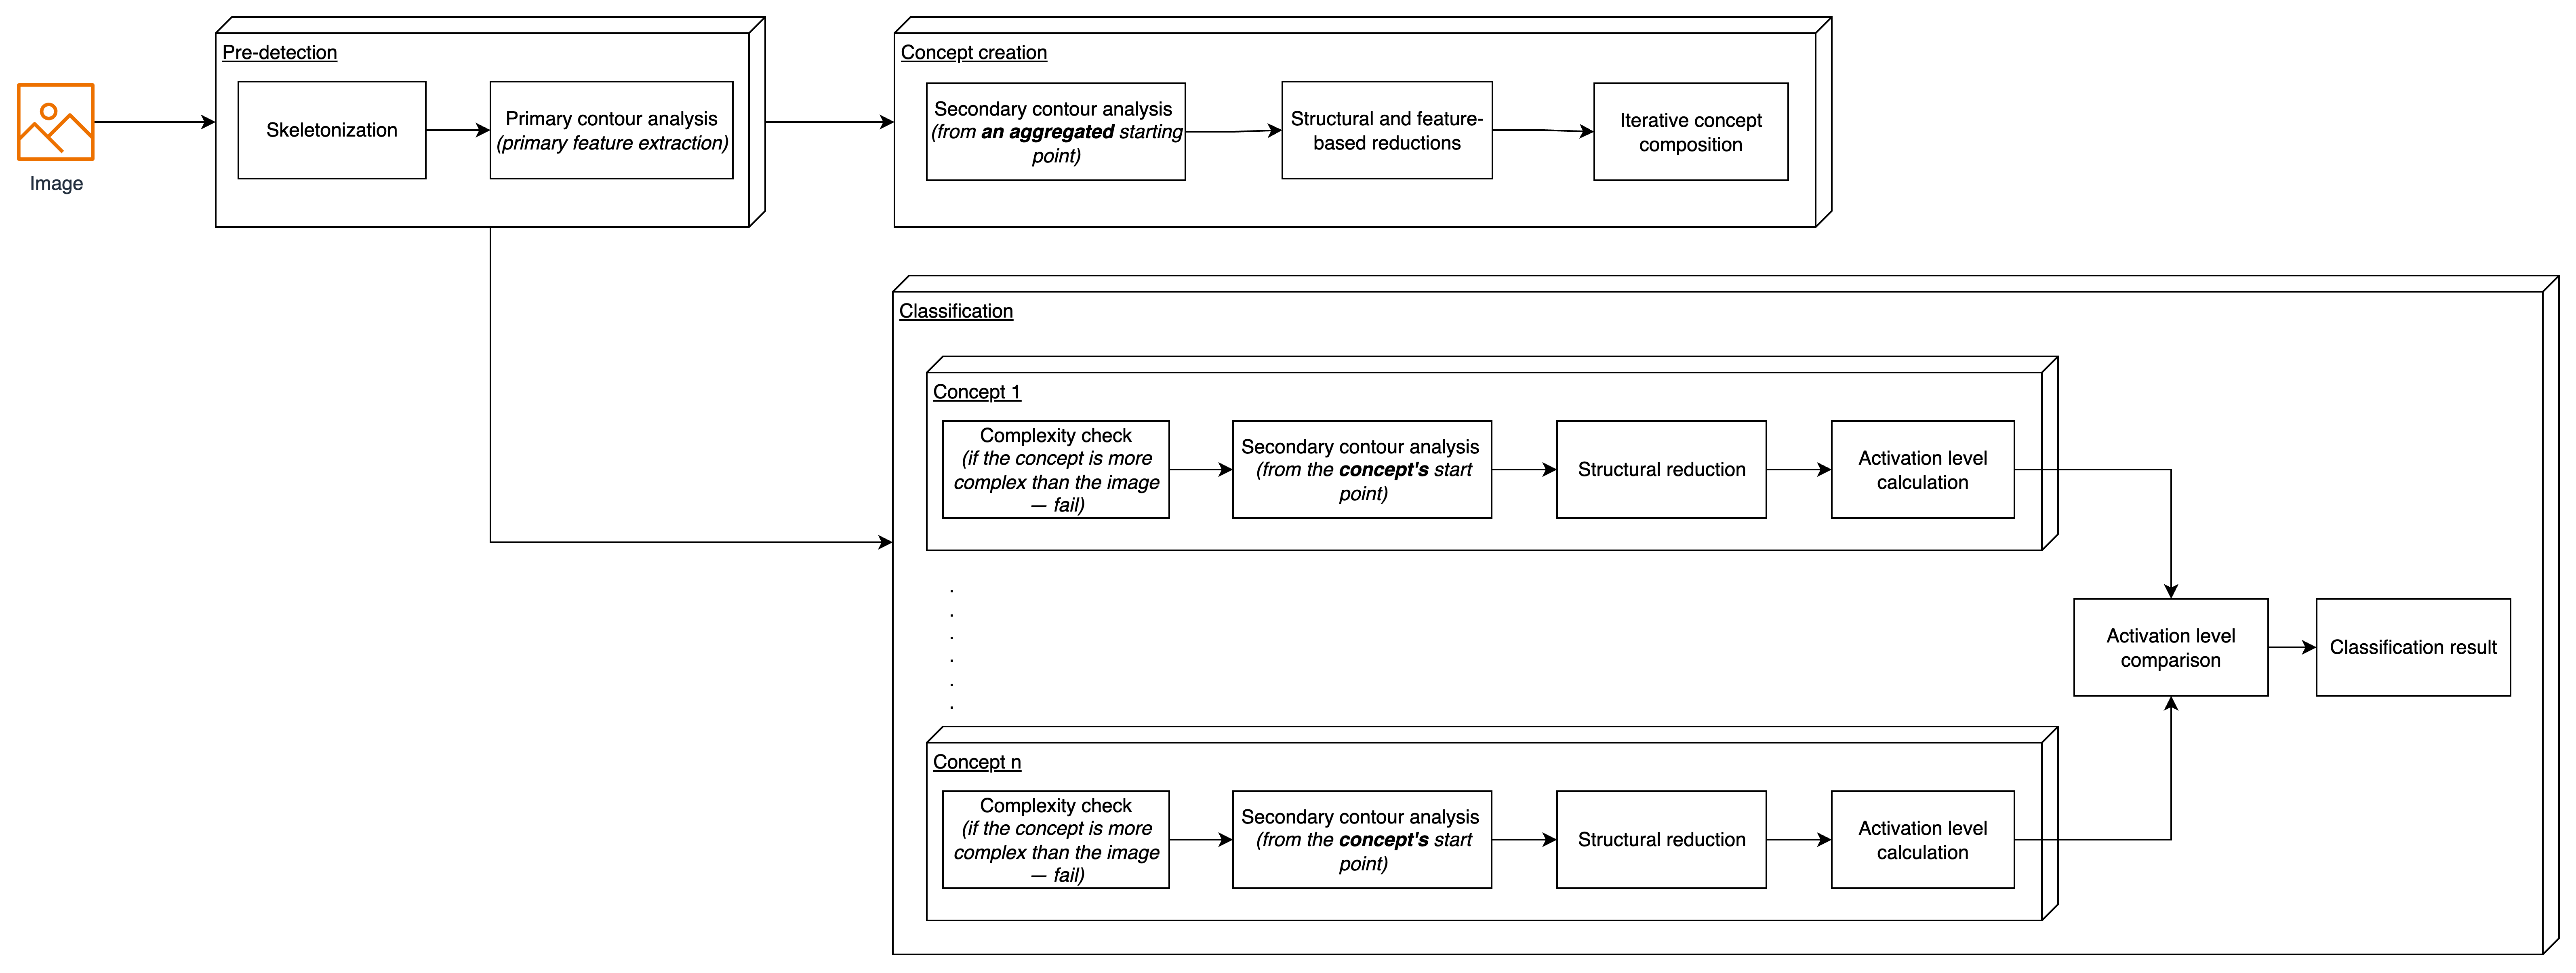
\includegraphics[width=\textwidth]{../../docs/images/basic_architecture.png}
\caption{ComAN system architecture showing pre-detection (skeletonization, primary analysis), concept formation (secondary analysis, reductions, iterative composition), and classification (complexity filtering, structural reduction, activation comparison).}
\label{fig:architecture}
\end{figure}

\subsection{Preprocessing: Skeletonization and Primary Contour Analysis}

The preprocessing stage transforms pixel-based images into graph-based structural representations through an eight-stage pipeline. This stage achieves edge-thickness invariance and topological preservation while extracting quantitative geometric features (implementation details in Section~4.1).

\textbf{Skeletonization Pipeline.} The system applies sequential transformations to extract a simplified graph from the input image:

\begin{enumerate}
\item \textbf{Adaptive Binary Thresholding:} Convert grayscale image $I(x,y)$ to binary $I_{\text{binary}}(x,y)$ using threshold $\theta$. To balance noise reduction with structural completeness, the system iteratively decreases $\theta$ until the resulting graph achieves connectivity, optimizing:
\[
\theta_{\text{optimal}} = \arg\max_{\theta} \{\theta : \text{connectivity}(G_{\theta}) = \text{true} \land \theta \geq \theta_{\text{min}}\}
\]

\item \textbf{Morphological Skeletonization:} Apply medial-axis transform to reduce binary regions to one-pixel-width curves while preserving topology.

\item \textbf{Branch Pruning:} Remove spurious skeleton branches to eliminate noise-induced artifacts.

\item \textbf{Point Cloud Extraction:} Convert skeleton pixels to a point cloud $P = \{p_1, p_2, \dots, p_m\}$ for graph-based processing.

\item \textbf{Topology Learning:} Apply Growing Neural Gas (GNG) \cite{fritzke1995} to learn topological connectivity from the point cloud, dynamically constructing a network that captures the skeleton's structure.

\item \textbf{Graph Simplification:} Reduce graph complexity using the Ramer--Douglas--Peucker algorithm, removing vertices below a perpendicular-distance threshold while preserving essential geometric features.

\item \textbf{Attributed Graph Construction:} Build graph $G = (V, E)$ with attributed nodes (point types, coordinates) and edges (geometric parameters).

\item \textbf{Coordinate Normalization:} Transform from absolute pixel coordinates to relative centered coordinates via $(x_{\text{norm}}, y_{\text{norm}}) = (x - x_{\text{centroid}}, y - y_{\text{centroid}})$, achieving translation invariance.
\end{enumerate}

Figure~\ref{fig:skeletonization} demonstrates the progressive transformation from grayscale input through binary thresholding, skeletonization, topology learning, and final simplified graph representation.

\begin{figure}[h]
\centering
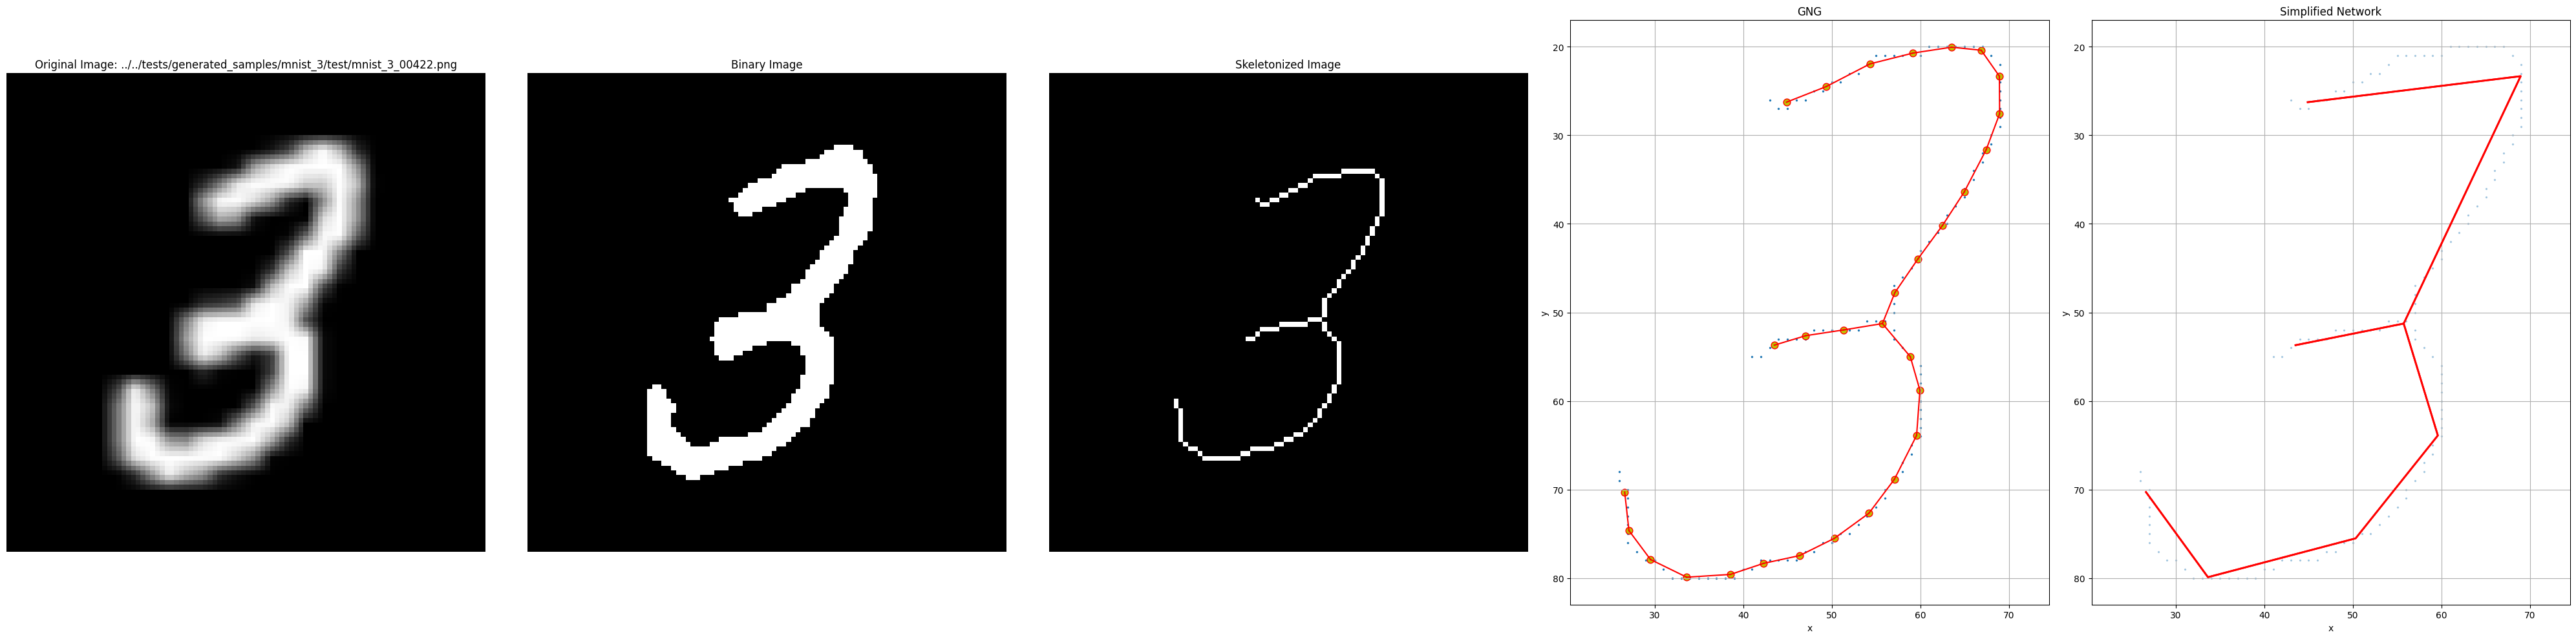
\includegraphics[width=\textwidth]{../../docs/images/skeletonization_example.png}
\caption{Skeletonization pipeline stages: (left to right) original MNIST digit, binary image after adaptive thresholding, morphological skeleton, GNG-learned graph, and RDP-simplified network.}
\label{fig:skeletonization}
\end{figure}

\textbf{Primary Contour Analysis.} After graph construction, the system classifies structural elements and extracts geometric parameters (detailed in Section~4.2). Nodes are typed based on degree and structural role: \texttt{EndPoint} ($\deg(v) = 1$), \texttt{CornerPoint} (degree-2 with significant angular change), \texttt{IntersectionPoint} ($\deg(v) \geq 3$), and generic \texttt{Point}. Edges are classified as \texttt{HorizontalLine} or \texttt{VerticalLine} based on projection magnitudes to the horizontal and vertical axes.

Parameters extracted include: for edges, endpoint coordinates, Euclidean length, orientation angle (discretized), quadrant location, and directional indicators; for nodes, centered coordinates, relative distance from structural centroid, incident angles, and spatial segments. Figure~\ref{fig:graph_sample} shows an annotated graph with labeled critical points and directional edge vectors.

\begin{figure}[h]
\centering
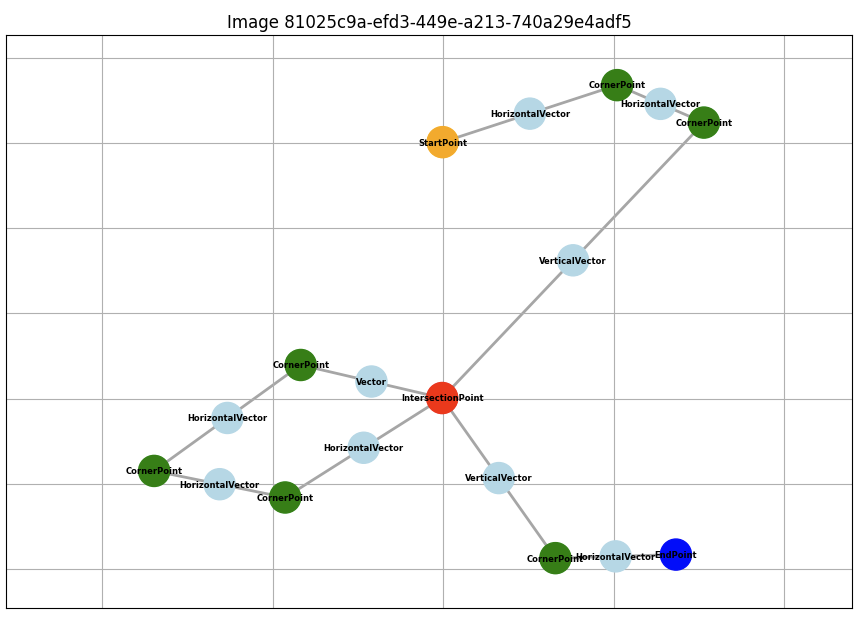
\includegraphics[width=0.8\textwidth]{../../docs/images/first_graph_sample.png}
\caption{Primary graph representation with annotated node types (orange: StartPoint, green: CornerPoint, red: IntersectionPoint, blue: EndPoint) and Line segments.}
\label{fig:graph_sample}
\end{figure}

\subsection{Concept Formation: Secondary Analysis and Reductions}

Concept formation constructs a canonical structural attractor $C$ from training graphs $\{G_1, G_2, \dots, G_n\}$ through iterative structural and parametric generalization. The process begins with selecting a stable reference frame, then applies reduction operators to extract common substructures (implementation in Section~4.3--4.4).

\textbf{Start Point Selection via Clustering.} To ensure consistent graph traversal across samples, the system identifies a stable starting node through adaptive clustering applied to normalized critical-point coordinates across all training samples. Clustering parameters adjust iteratively based on cluster quality metrics, with epsilon and minimum sample count scaled relative to the dataset size and spatial distribution. The system classifies structure type as OPEN (if any sample contains an \texttt{EndPoint}) or CLOSED, influencing subsequent reduction strategies.

\textbf{Structural Reduction Hierarchy.} The system defines type hierarchies enabling progressive simplification:
\begin{itemize}
\item \textbf{Point hierarchy:} \texttt{IntersectionPoint} $\rightarrow$ \texttt{CornerPoint} $\rightarrow$ \texttt{Point}
\item \textbf{Edge hierarchy:} \texttt{VerticalLine}/\texttt{HorizontalLine} $\rightarrow$ \texttt{Line}
\end{itemize}

Type-based reduction rules downgrade node types based on structural context: an \texttt{IntersectionPoint} reduces to \texttt{EndPoint} if degree falls to 1 after edge removal, or to \texttt{CornerPoint} if degree no longer matches the expected intersection count. These transformations maintain topological consistency while generalizing structure.

\textbf{EndPoint Reduction Algorithm.} To align endpoint counts between concept and new sample, the system applies a dual-phase algorithm:
\begin{enumerate}
\item \textbf{Similarity-based removal:} Compute pairwise similarity matrix $S$ between concept endpoints $E_{\text{concept}}$ and image endpoints $E_{\text{image}}$. Remove endpoints with maximum similarity below a noise-filtering threshold.
\item \textbf{Count balancing:} If $|E_{\text{image}}| > |E_{\text{concept}}|$, compute excess $\Delta = |E_{\text{image}}| - |E_{\text{concept}}|$ and remove the $\Delta$ endpoints with lowest similarity scores.
\end{enumerate}

For each removed endpoint, the system traces a path to the nearest critical point (intersection or corner) and deletes all intervening nodes, preserving topological integrity. Endpoint detection uses the criterion: $\text{IsEndPoint}(v) = \text{true}$ if $\deg(v) = 1 \land v \notin \text{StartPoints}$.

\textbf{Iterative Composition.} Concept formation proceeds incrementally:
\begin{align*}
C_0 &= G_1 \\
C_{i+1} &= \mathcal{A}(C_i, G_{i+1}), \quad i = 1, 2, \dots, n-1
\end{align*}
where $\mathcal{A}$ denotes the attractor-formation operator that: (1) reduces $G_{i+1}$ to match $C_i$'s structure, (2) generalizes $C_i$'s parameters through range expansion and set intersection, and (3) updates $C_i$ with the merged representation. Training terminates after processing all samples; the current implementation does not employ dynamic stabilization criteria (see Section~4.4 for parameter generalization mechanisms). Figure~\ref{fig:concept_formation} illustrates four iterations of concept formation for MNIST digit ``3'', showing progressive endpoint removal, intersection-to-corner reduction, and parameter range expansion.

\begin{figure}[h]
\centering
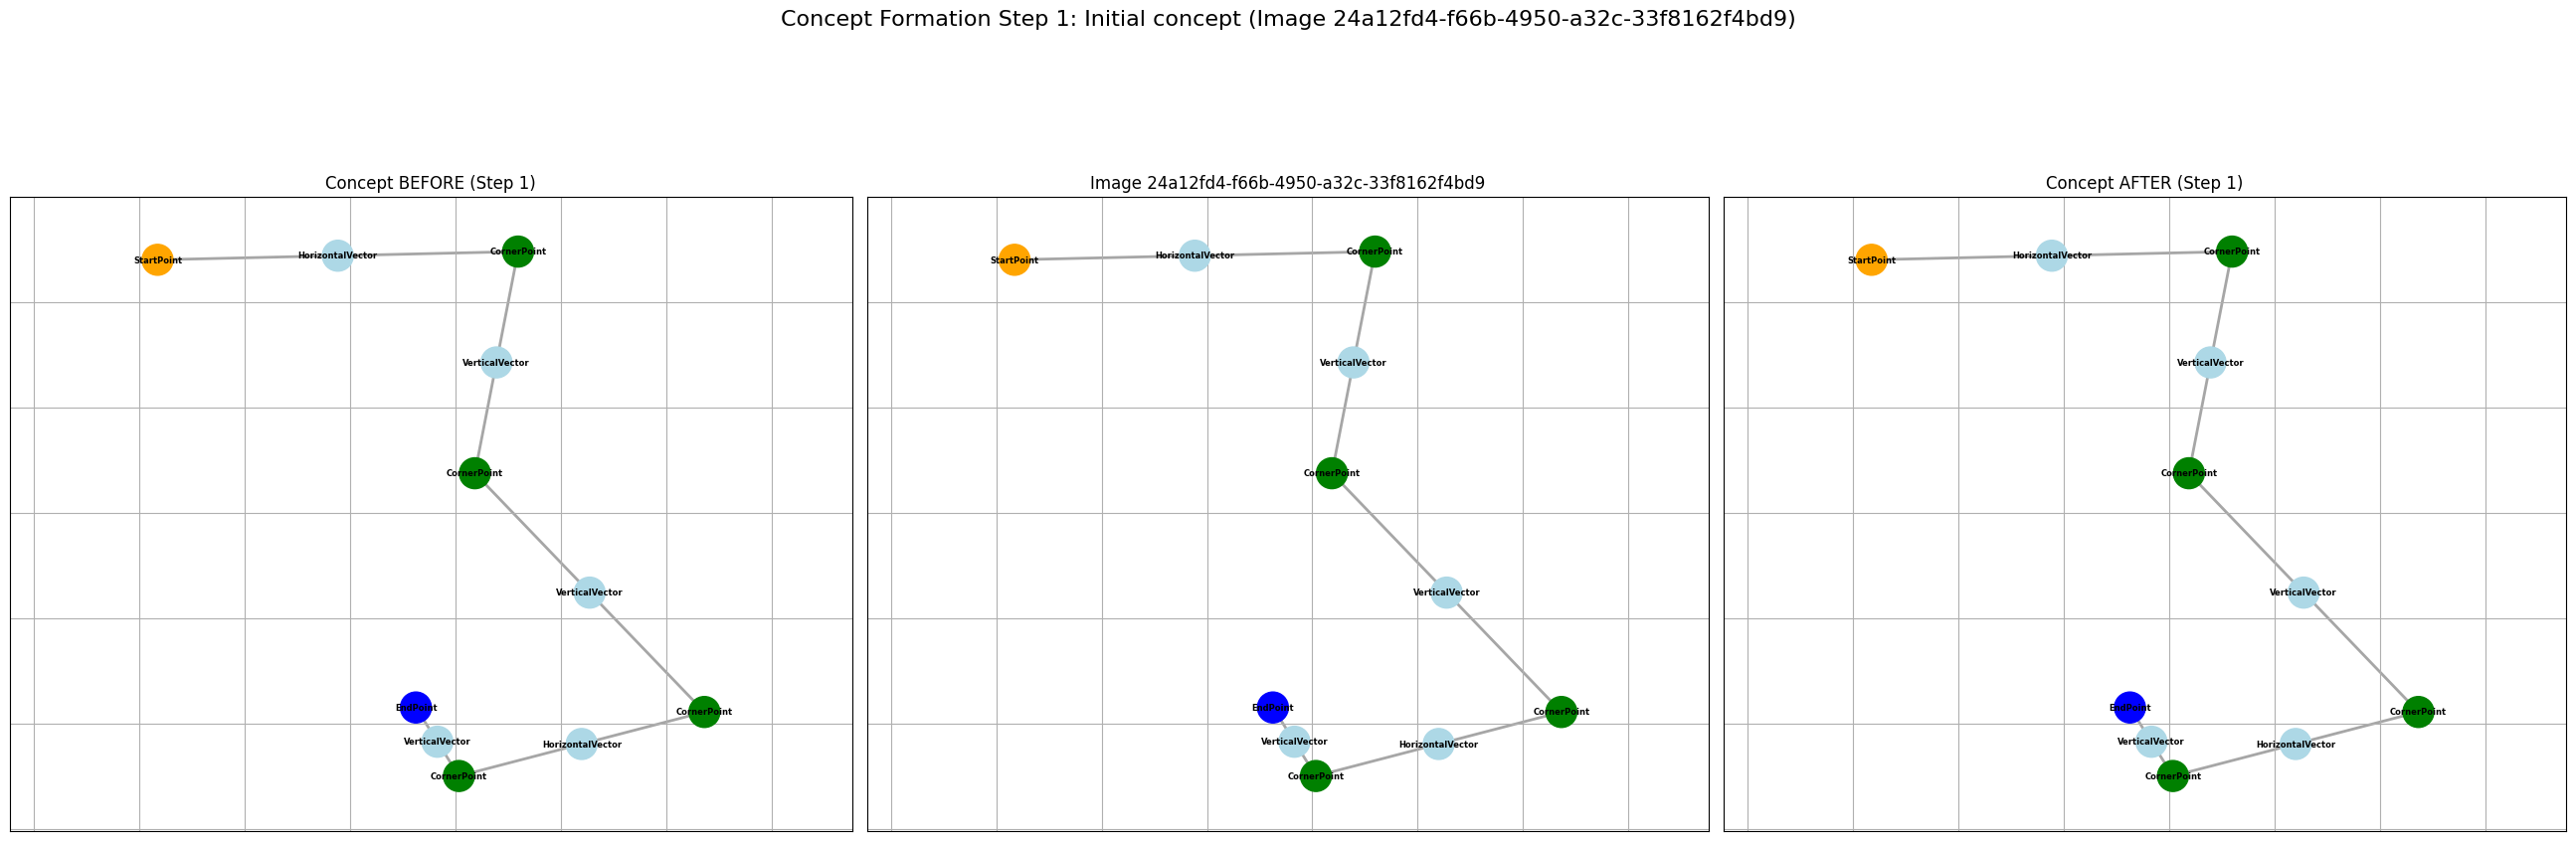
\includegraphics[width=0.45\textwidth]{../../docs/images/concept_formation/step_1.png}
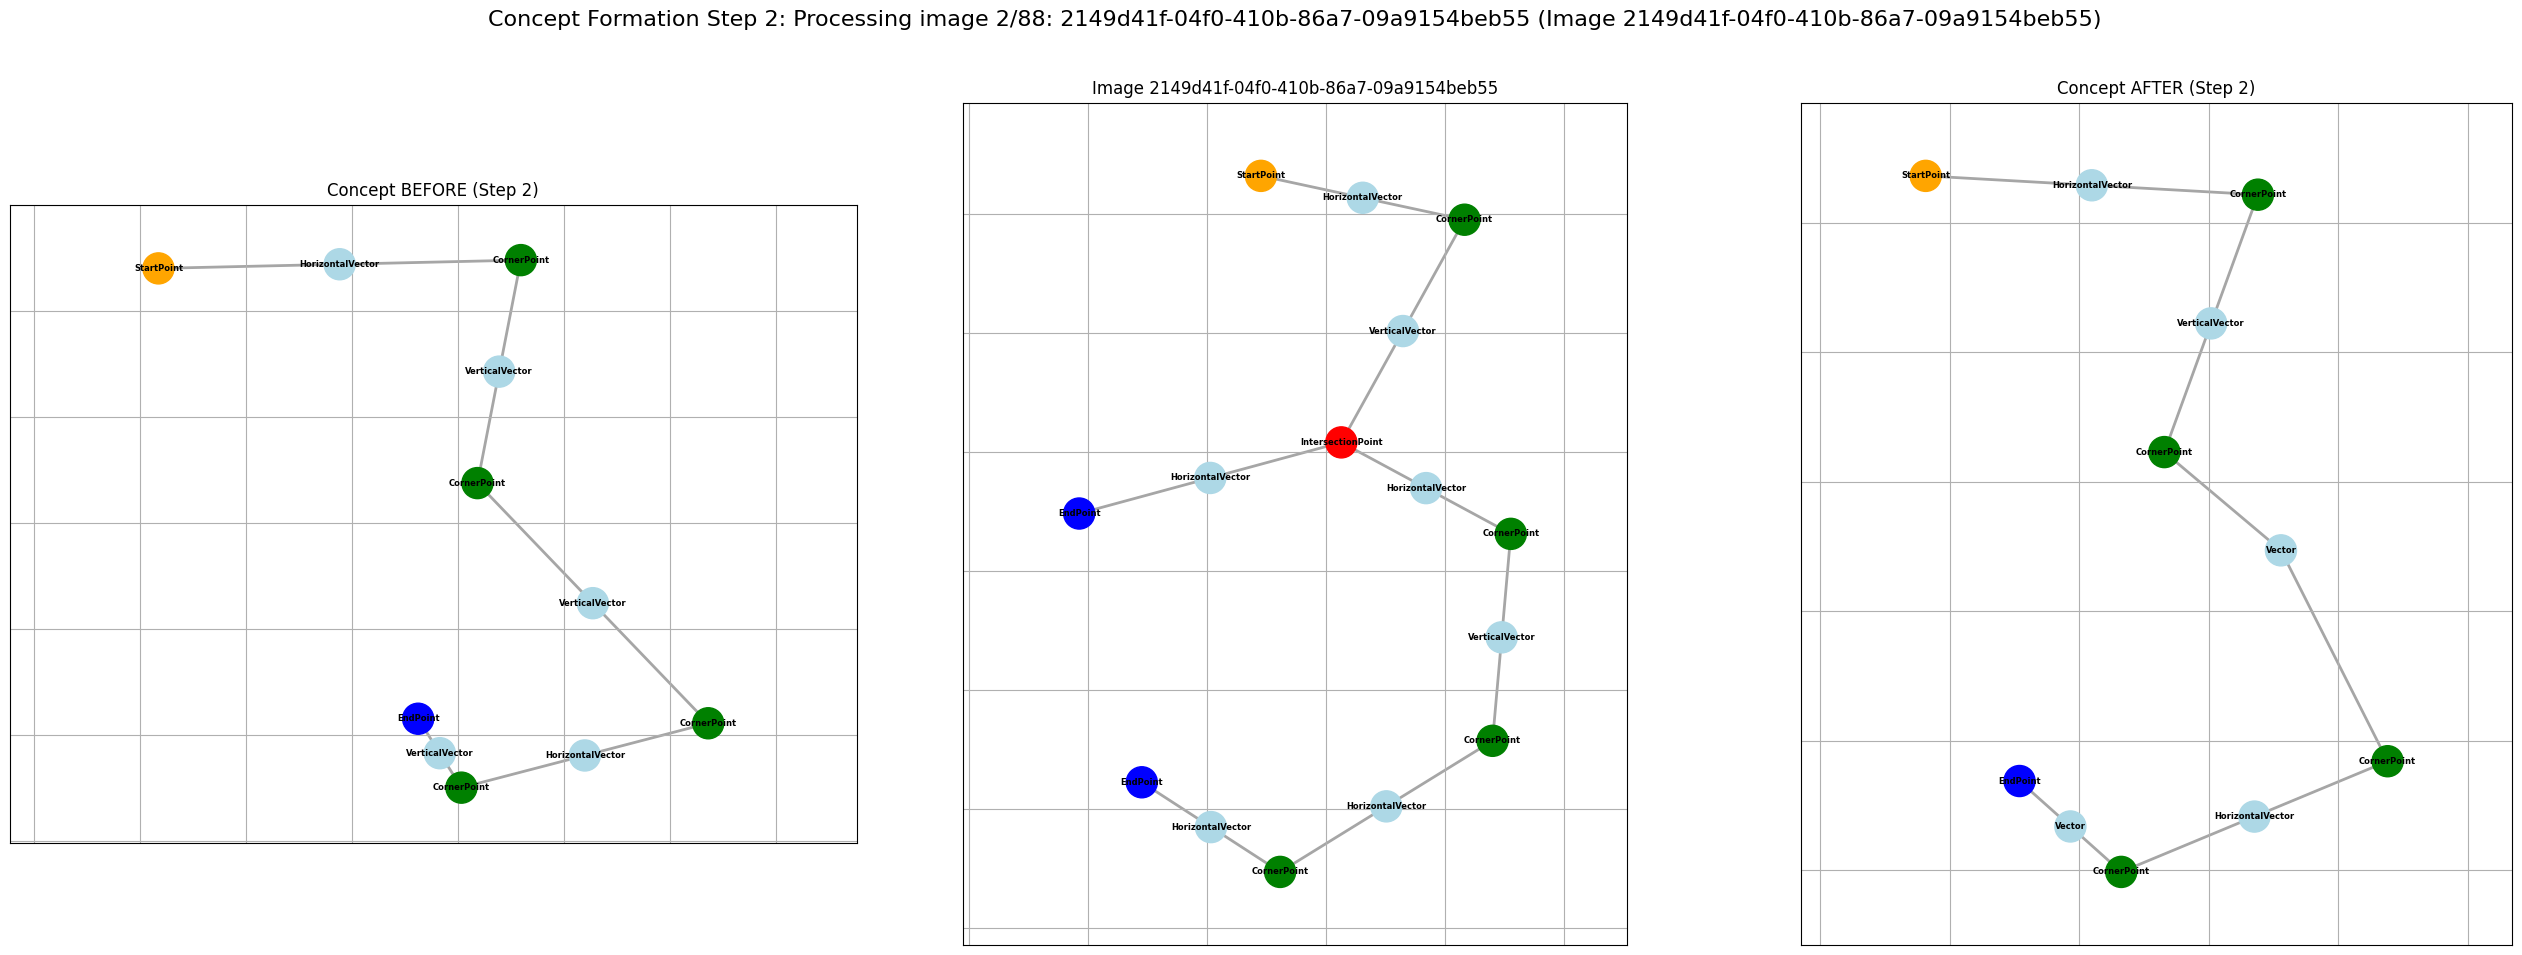
\includegraphics[width=0.45\textwidth]{../../docs/images/concept_formation/step_2.png} \\
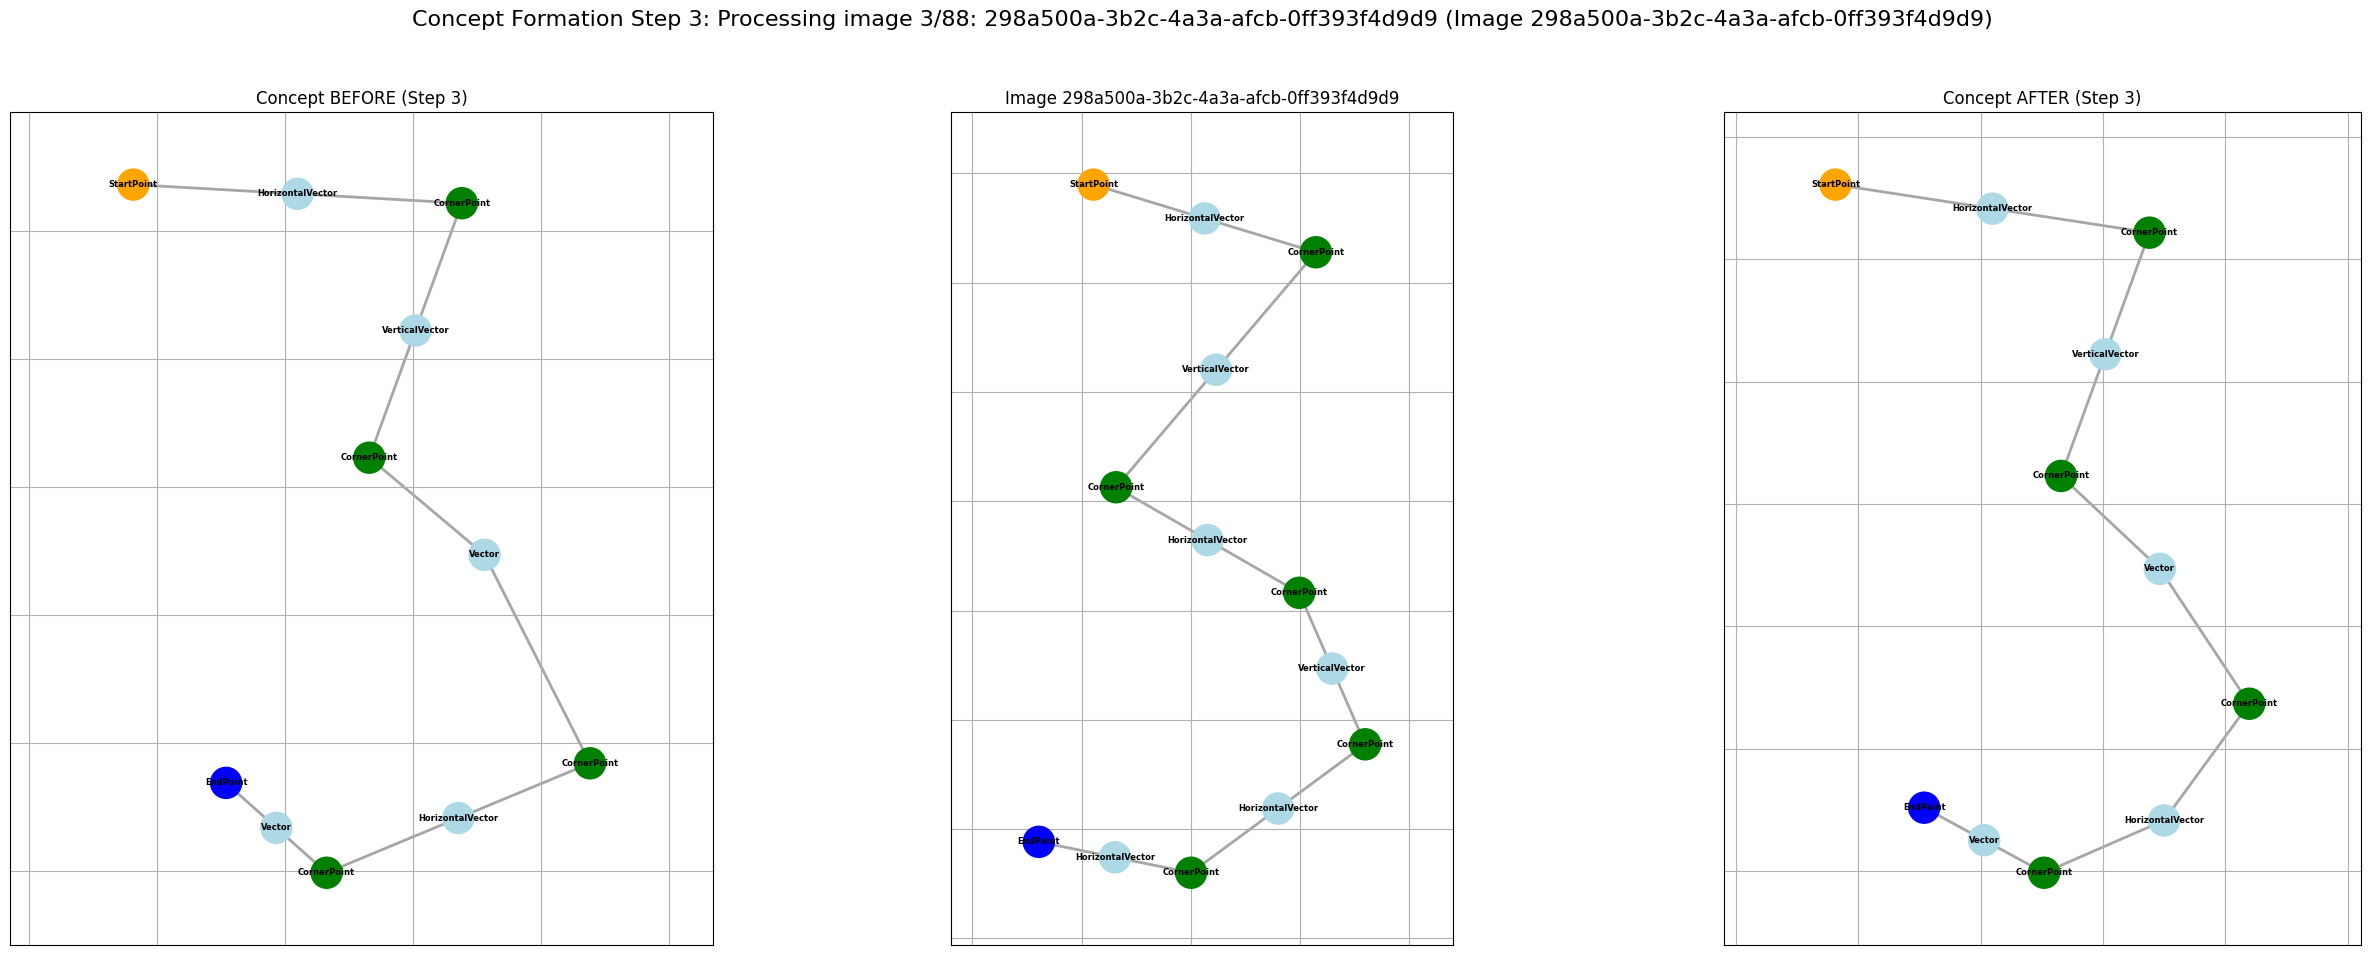
\includegraphics[width=0.45\textwidth]{../../docs/images/concept_formation/step_3.png}
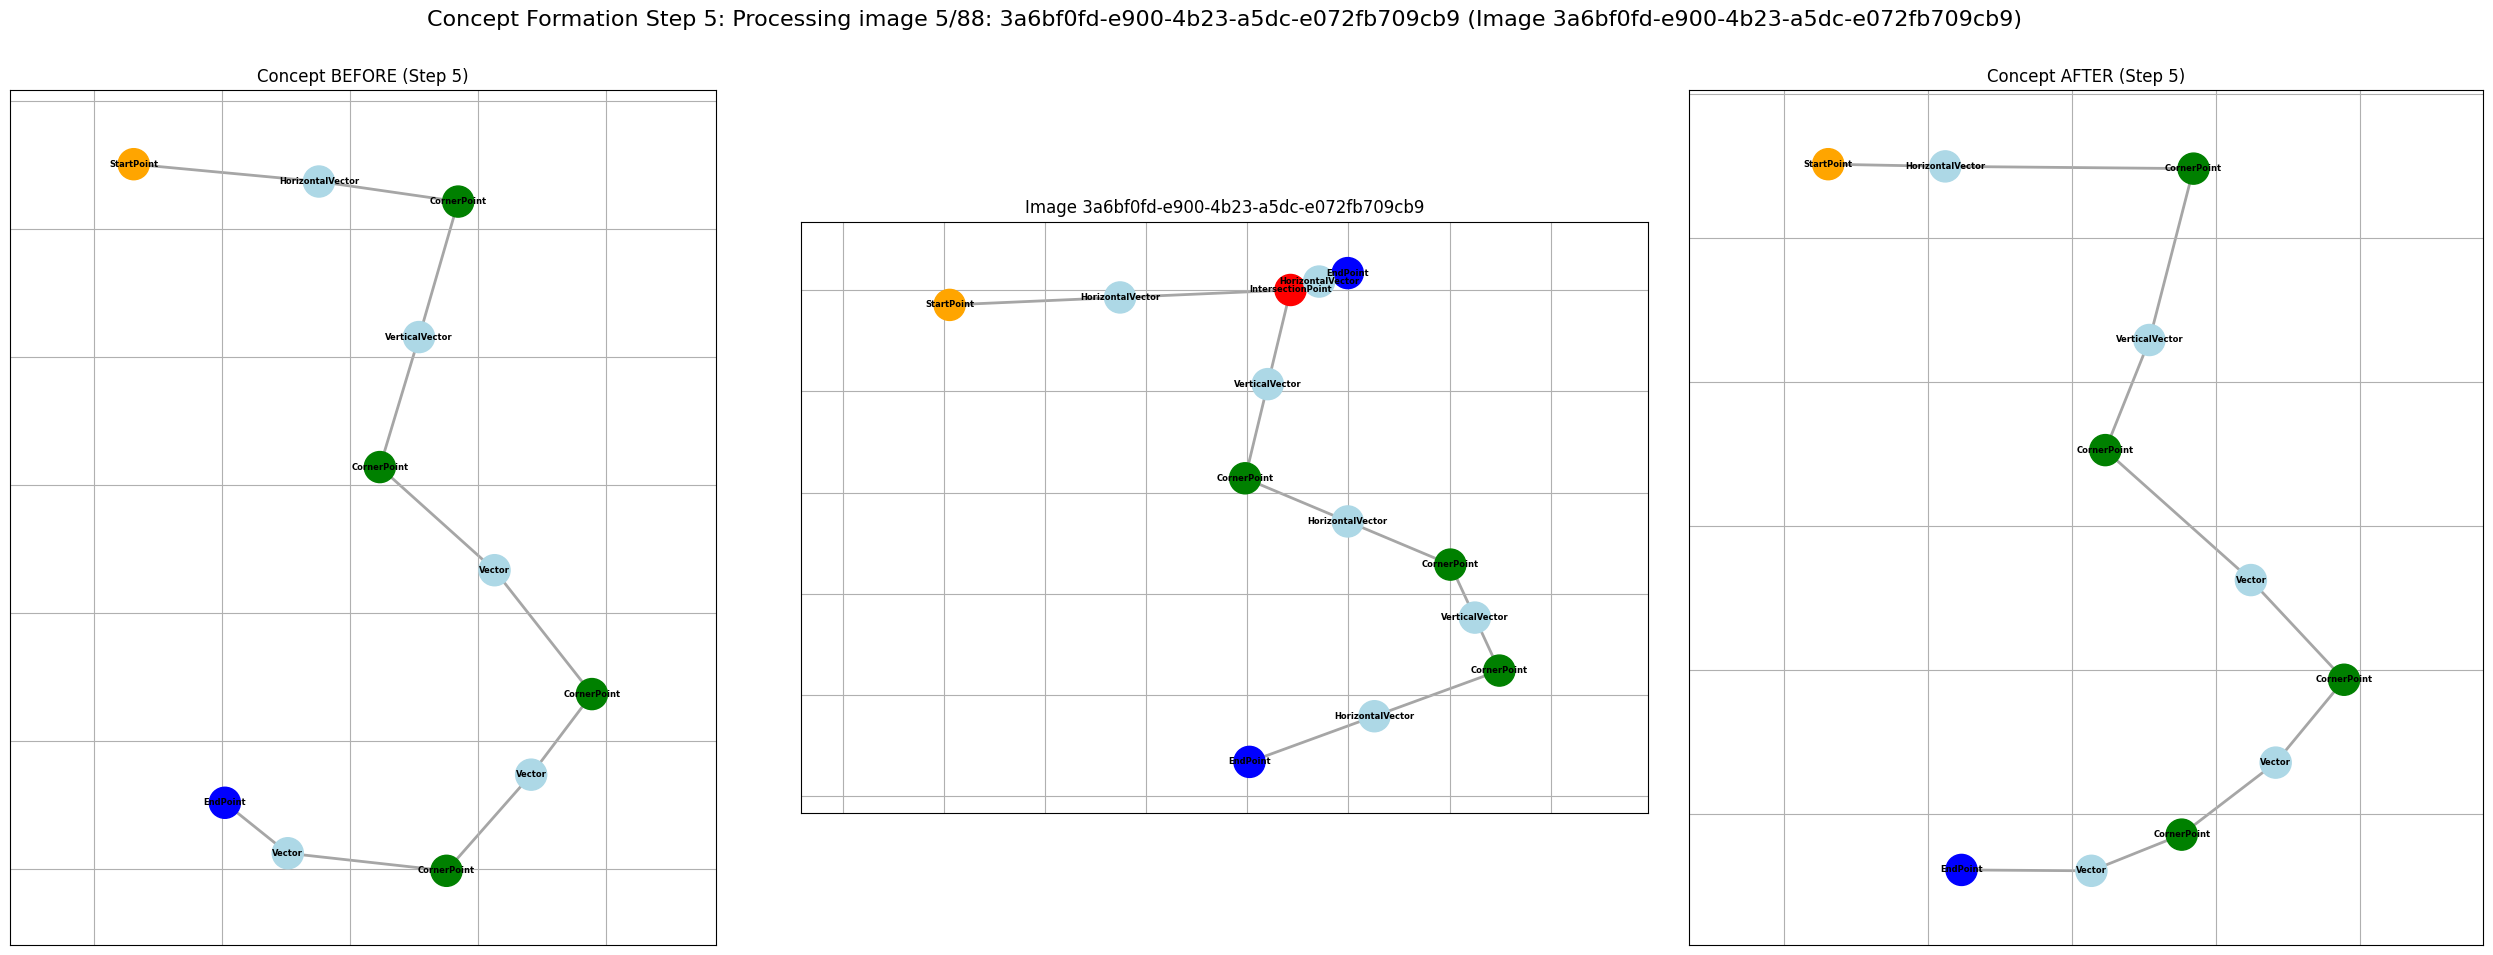
\includegraphics[width=0.45\textwidth]{../../docs/images/concept_formation/step_4.png}
\caption{Concept formation progression for digit ``3'': (top-left) initial seed $C_0 = G_1$; (top-right) iteration 2 removes redundant endpoint, reduces IntersectionPoint to CornerPoint; (bottom-left) iteration 3 removes lower corner point; (bottom-right) iteration 4 eliminates noise substructure.}
\label{fig:concept_formation}
\end{figure}

\subsection{Classification and Decision}

Classification treats inference as iterative reduction of the test graph $G_{\text{test}}$ toward stored concept attractors $\{C_1, C_2, \dots, C_N\}$, measuring proximity via Graph Edit Distance and selecting the nearest attractor through Winner-Takes-All competition.

\textbf{Multi-Stage Classification Pipeline.} For each concept $C_i$, the system executes:

\begin{enumerate}
\item \textbf{Complexity Filter:} Reject $C_i$ if $\text{complexity}(C_i) > \text{complexity}(G_{\text{test}})$, where $\text{complexity}(G) = |V(G)| + |E(G)|$. This early-rejection mechanism prevents matching a structurally richer concept to a simpler test graph.

\item \textbf{Start Point Alignment:} Identify the optimal start node $s_{\text{concept}}$ in $C_i$, locate the corresponding node $s_{\text{image}}$ in $G_{\text{test}}$, and reorder traversal to ensure consistent structural comparison.

\item \textbf{Feature Enhancement:} Apply visitor patterns (\texttt{AngleVisitor}, \texttt{QuadrantVisitor}, \texttt{DirectionVisitor}) to compute secondary geometric features required for parametric matching.

\item \textbf{Critical Point Reduction:} Sequentially apply \texttt{EndpointReduction}, \texttt{IntersectionReduction}, and \texttt{CornerPointReduction} strategies to align $G_{\text{test}}$ with $C_i$'s structure, producing reduced graph $G_{\text{reduced}}$.

\item \textbf{Graph Edit Distance Computation:} Calculate $\text{GED}(G_{\text{reduced}}, C_i)$ as the minimum-cost sequence of edit operations (node/edge substitution, insertion, deletion) transforming $G_{\text{reduced}}$ into $C_i$.
\end{enumerate}

\textbf{Activation Metric.} Similarity between the test graph and concept $C_i$ is computed as:
\[
\text{similarity}_i = 1.0 - \frac{\text{GED}(G_{\text{reduced}}, C_i)}{\text{max\_possible\_cost}}
\]
where $\text{max\_possible\_cost} = \max(|V_{\text{image}}| + |V_{C_i}|, 1)$ provides scale-invariant normalization. The GED cost function is structured to prioritize structural over parametric mismatches: node operations are weighted more heavily than edge operations (structural primacy), and property compatibility determines substitution costs. Specifically, node label incompatibility results in infinite cost (enforcing type constraints), while compatible nodes incur costs based on property differences. Numeric properties use tolerance-based comparison to avoid floating-point artifacts; range properties measure distance from acceptable bounds; list properties require subset containment (detailed cost structure in Section~4.3).

\textbf{Winner-Takes-All Decision.} After computing similarity scores for all viable concepts, the system filters results retaining only structurally valid matches, sorts by similarity (descending), and applies complexity-based tie-breaking: if multiple concepts achieve identical similarity $s$, the concept with maximum $|V| + |E|$ wins, reflecting greater structural specificity. For example, if concepts $C_{\text{eight}}$, $C_{\text{zero}}$, and $C_{\text{infinity}}$ all achieve similarity 0.84, the system selects $C_{\text{eight}}$ with complexity 17 over $C_{\text{infinity}}$ (complexity 15) and $C_{\text{zero}}$ (complexity 13).

\subsection{Data Flow Summary}

Table~\ref{tab:dataflow} summarizes the stage-by-stage transformations, input/output representations, and key data structures throughout the ComAN pipeline.

\begin{table}[h]
\centering
\caption{ComAN pipeline data flow and transformations.}
\label{tab:dataflow}
\begin{tabular}{p{2.5cm}p{2.2cm}p{4cm}p{2cm}p{3.5cm}}
\toprule
\textbf{Stage} & \textbf{Input} & \textbf{Operations} & \textbf{Output} & \textbf{Key Structures} \\
\midrule
Skeletonization & Grayscale image & Adaptive threshold $\rightarrow$ skeleton $\rightarrow$ GNG $\rightarrow$ RDP & Graph $G(V,E)$ & NetworkX graph, node/edge attributes \\
\midrule
Primary Analysis & Graph $G$ & Type classification, parameter extraction & Annotated graph & Point/Line type labels, geometric params \\
\midrule
Concept Formation & Training graphs $\{G_1 \dots G_n\}$ & Start selection, reduction, composition & Concept $C$ & Hypergraph attractor with parameter ranges \\
\midrule
Classification & Test graph $G_{\text{test}}$ & Complexity filter, reduction, GED & Class label + similarity & Similarity matrix, edit path \\
\bottomrule
\end{tabular}
\end{table}

\newpage

\section{Practical Implementation of Components}

\subsection{Skeletonization and Graph Construction}

The skeletonization pipeline uses established libraries chosen for reliability and functionality.

\textbf{Library Selection and Rationale.} The implementation employs \texttt{scikit-image} for morphological operations (widely-used, well-tested skeletonization algorithms), \texttt{skan} for branch pruning (specialized library for skeleton analysis), and \texttt{NetworkX} for graph representation (flexible Python library with rich attribute support). This combination balances standard computer vision tools with graph-theoretic data structures.

\textbf{Algorithmic Choices.} For morphological skeletonization, we employ scikit-image's \texttt{skeletonize} function, which implements Zhang--Suen thinning algorithm. To remove spurious short branches that arise from noise, we apply post-processing using the skan library: branches shorter than 7 pixels connecting junctions to endpoints are pruned. The adaptive thresholding strategy starts with a high initial threshold to minimize noise, then iteratively decreases the threshold (typical decrements of 5 units) until the resulting graph achieves connectivity, with a minimum threshold preventing excessive noise inclusion.

\textbf{Complexity Analysis.} The pipeline complexity comprises: (1) morphological operations: $O(n \cdot m)$ for an $n \times m$ image; (2) GNG topology learning: $O(k \cdot |P|)$ where $k$ is the iteration count and $|P|$ is the number of skeleton points; (3) RDP simplification: $O(|V|^2)$ worst-case, typically $O(|V| \log |V|)$ for simple curves. Overall preprocessing complexity is $O(n \cdot m + k \cdot |P|)$, dominated by morphological operations for typical images.

\textbf{Data Structure Schema.} The NetworkX graph stores node attributes including: \texttt{point\_type} (EndPoint, CornerPoint, IntersectionPoint, Point), \texttt{x} and \texttt{y} coordinates (both absolute and normalized), \texttt{relative\_distance}, \texttt{angle} (for corners/intersections), and \texttt{segments} (spatial location list). Edge attributes include: \texttt{line\_type} (HorizontalLine, VerticalLine, Line), \texttt{length}, \texttt{angle\_with\_origin}, \texttt{quadrant}, \texttt{horizontal\_direction}, and \texttt{vertical\_direction}. All parametric values are stored as either single values or ranges (min/max pairs) for concept graphs.

\textbf{Parameter Selection.} GNG hyperparameters affect graph quality: learning rate controls how quickly nodes adapt to the skeleton structure, maximum node count limits graph complexity, and insertion frequency determines granularity. RDP epsilon balances simplification (higher epsilon removes more vertices) versus feature preservation (lower epsilon retains detail). Current parameter values are empirically tuned for MNIST-scale images and available in the implementation repository.

\subsection{Primary Contour Analysis}

After graph construction, the system extracts geometric and topological features through visitor pattern-based traversals.

\textbf{Node Type Classification.} The classification logic applies degree-based rules:
\begin{itemize}
\item $\deg(v) = 1 \land v \notin \text{StartPoints} \Rightarrow$ \texttt{EndPoint}
\item $\deg(v) = 2 \land \text{angle}(v) > \theta_{\text{corner}} \Rightarrow$ \texttt{CornerPoint}
\item $\deg(v) \geq 3 \Rightarrow$ \texttt{IntersectionPoint}
\item Otherwise $\Rightarrow$ generic \texttt{Point}
\end{itemize}
where $\theta_{\text{corner}}$ defines the minimum angular deviation to qualify as a corner (avoiding trivial directional changes).

\textbf{Edge Classification.} Edges are classified by projection magnitudes: if $|x_2 - x_1| > |y_2 - y_1|$, the edge is \texttt{HorizontalLine}; otherwise \texttt{VerticalLine}. This classification provides coarse orientation information independent of absolute angle values.

\textbf{Parameter Enumeration.} Table~\ref{tab:parameters} lists extracted parameters, their data types, and purposes.

\begin{table}[h]
\centering
\caption{Extracted geometric and topological parameters.}
\label{tab:parameters}
\begin{tabular}{lllp{5cm}}
\toprule
\textbf{Element} & \textbf{Parameter} & \textbf{Type} & \textbf{Purpose} \\
\midrule
Edge & \texttt{angle\_with\_origin} & float & Orientation encoding relative to horizontal axis \\
Edge & \texttt{quadrant} & int \{1,2,3,4\} & Coarse spatial location \\
Edge & \texttt{length} & float & Geometric magnitude \\
Node & \texttt{segments} & list & Multi-valued spatial descriptor (TOP, BOTTOM, LEFT, RIGHT) \\
Node & \texttt{relative\_distance} & float & Distance from structural centroid \\
\bottomrule
\end{tabular}
\end{table}

\textbf{Coordinate Transformations.} The transformation from absolute (SC$_A$) to relative (SC$_R$) coordinates uses the centroid formula:
\[
\bar{x} = \frac{1}{|V|}\sum_{v \in V} x_v, \quad \bar{y} = \frac{1}{|V|}\sum_{v \in V} y_v
\]
\[
x_{\text{rel}} = x - \bar{x}, \quad y_{\text{rel}} = y - \bar{y}
\]
This centering achieves translation invariance, ensuring that shifting the image does not affect relative geometric relationships.

\textbf{Discretization Trade-offs.} Angular discretization (e.g., into bins) increases invariance to small rotations but reduces specificity. Finer bins (smaller step sizes) preserve more orientation information but decrease generalization across rotated instances of the same class. The discretization granularity represents a tunable trade-off between rotation robustness and discriminative power.
\subsection{Secondary Analysis and Reductions}

The reduction phase aligns training samples and test images to stored concept structures through structural simplification and parametric matching.

\textbf{Clustering Algorithm Selection.} Start point selection employs multiple clustering strategies depending on dataset characteristics: DBSCAN for dense, uniformly-distributed critical points; OPTICS for variable-density clusters where different regions have different point concentrations; Agglomerative clustering with Ward linkage as a fallback when density-based methods fail. Parameters are adapted iteratively: epsilon and minimum sample count are scaled relative to the total sample count and the spatial distribution variance of critical points across training images.

\textbf{GED Cost Structure.} The Graph Edit Distance cost function embodies design principles rather than fixed values. Node operations are weighted substantially more heavily than edge operations (approximately 10:1 ratio) to prioritize structural accuracy over path details. Edge costs are set lower to allow flexible matching of connection patterns. The cost design ensures that structural mismatches (wrong node types, incompatible topology) dominate the distance metric, while parametric differences (slightly different angles or positions) contribute proportionally.

Property-specific cost functions follow these principles:
\begin{itemize}
\item \textbf{Numeric properties} (coordinates, angles): Use tolerance-based comparison to prevent floating-point comparison artifacts. Values within tolerance are treated as equal (zero cost); values outside tolerance incur fixed cost.
\item \textbf{Range properties}: When a concept parameter is generalized to a range $[R_{\min}, R_{\max}]$, test values within the range incur cost proportional to distance from the range center (rewarding central values); values outside the range incur maximum cost.
\item \textbf{List properties} (segments, directions): Require subset containment---concept lists must be subsets of image lists. If $L_c \subseteq L_i$, cost is zero; otherwise maximum cost.
\end{itemize}

The relative cost magnitudes are empirically tuned; current values are available in the codebase.

\textbf{Endpoint Reduction Pseudocode.} Algorithm~\ref{alg:endpoint} details the endpoint path-finding and removal process.

\begin{algorithm}
\caption{Endpoint Reduction via Path Removal}
\label{alg:endpoint}
\begin{algorithmic}[1]
\Require Graph $G$, endpoint $e$ to remove
\Ensure Modified graph $G'$ with $e$ and its path removed
\State $\text{path} \gets [e]$
\State $\text{current} \gets e$
\While{$\deg(\text{current}) = 1$ AND $\text{current} \notin \text{CriticalPoints}$}
    \State $\text{neighbors} \gets \text{GetNeighbors}(G, \text{current})$
    \State $\text{next} \gets \text{neighbors}[0]$ \Comment{Single neighbor for degree-1 node}
    \State $\text{path.append}(\text{next})$
    \State $\text{current} \gets \text{next}$
\EndWhile
\State $G' \gets G$
\ForAll{$v \in \text{path}[:-1]$} \Comment{Exclude final critical point}
    \State $G' \gets G' \setminus \{v\}$ \Comment{Remove node and incident edges}
\EndFor
\State \Return $G'$
\end{algorithmic}
\end{algorithm}

\textbf{Structural Validity Filtering.} The system applies structural constraints to filter invalid matches: concepts whose complexity (node + edge count) exceeds the test image complexity are rejected early; matches must preserve degree constraints at critical points; and connectivity must be maintained throughout reductions.

\subsection{Iterative Composition of Concepts}

The attractor formation operator generalizes concept parameters while preserving structural integrity.

\textbf{Parameter Generalization Strategies.} The system applies type-specific generalization:
\begin{itemize}
\item \textbf{Numeric values $\rightarrow$ ranges}: Track minimum and maximum values observed across all training samples. Initially, $C_0$ contains single values; after processing $n$ samples, each numeric parameter becomes $[\min_{i=1}^n v_i, \max_{i=1}^n v_i]$.
\item \textbf{Categorical values $\rightarrow$ set intersection}: Retain only labels/categories present in all training samples. For example, if sample 1 has direction "RIGHT" and sample 2 has "LEFT", the intersection is empty and the parameter is removed.
\item \textbf{List values $\rightarrow$ set intersection}: Preserve only elements common to all samples. If sample 1 has segments ["TOP", "RIGHT"] and sample 2 has ["TOP", "LEFT"], the concept retains ["TOP"].
\end{itemize}

\textbf{Attractor Persistence.} Concepts are stored as attributed NetworkX graphs (in-memory during training) or serialized to disk/database for long-term storage. Neo4j graph database provides an alternative storage backend when large concept repositories require persistent, queryable storage. Each concept graph includes: structural topology ($V$, $E$), node/edge type labels, and parametric ranges/sets for all extracted features.

\textbf{Training Termination.} The current implementation uses exhaustive training: concept formation continues until all training samples are processed. No dynamic convergence detection is employed. A potential future enhancement would monitor the graph edit distance between successive concept states: $\text{GED}(C_i, C_{i+1}) < \epsilon_{\text{conv}}$ would indicate stabilization, allowing early termination when additional samples no longer significantly modify the concept structure.

\section{Experimental Results}

To validate the ComAN architecture, we conducted controlled experiments on a subset of the MNIST handwritten digit dataset, focusing on few-shot learning scenarios with minimal training data.

\subsection{Experimental Setup}

\textbf{Dataset.} We selected 6 structurally diverse digit classes from MNIST: 1, 2, 3, 6, 7, and 9. These digits exhibit varying topological complexity (open vs. closed structures, different numbers of endpoints and intersections). The test set comprised the standard MNIST test split filtered to these six classes, totaling 4,734 images.

\textbf{Training Scenarios.} To evaluate ComAN's few-shot learning capability, we designed four training configurations:
\begin{itemize}
\item \textbf{No Augmentation:} 5--6 unique base samples per class (45 total samples)
\item \textbf{+2 Augmentation:} Base samples plus 2 augmented variants each (135 total)
\item \textbf{+5 Augmentation:} Base samples plus 5 augmented variants each (270 total)
\item \textbf{+10 Augmentation:} Base samples plus 10 augmented variants each (495 total)
\end{itemize}

Augmentation consisted of small rotations ($\pm 5^\circ$), translations ($\pm 2$ pixels), and elastic deformations to increase structural variability while preserving digit identity. Critically, all scenarios used only 5--6 \emph{unique} exemplars per class---augmentation provided additional instances of the same underlying forms.

\textbf{Implementation.} The system was implemented in Python using scikit-image for preprocessing, NetworkX for graph manipulation, and NetworkX's built-in graph matching for GED computation (Section~4). Training performed a single forward pass through all samples per class (no backpropagation, no multiple epochs). Classification evaluated all 4,734 test images against the learned concept base.

\subsection{Classification Performance}

Table~\ref{tab:results} presents classification metrics across all four training scenarios.

\begin{table}[h]
\centering
\caption{Classification performance on 4,734 test images across training scenarios.}
\label{tab:results}
\begin{tabular}{lcccccc}
\toprule
\textbf{Scenario} & \textbf{Training} & \textbf{Success} & \textbf{Accuracy} & \textbf{Precision} & \textbf{Recall} & \textbf{F1-Score} \\
 & \textbf{Samples} & \textbf{Rate} & (\%) & (\%) & (\%) & (\%) \\
\midrule
No Augmentation & 45 & 99.19 & 63.63 & 67.99 & 63.63 & 62.57 \\
+2 Augmentation & 135 & 99.30 & 69.54 & 78.83 & 69.54 & 66.01 \\
+5 Augmentation & 270 & 99.51 & 71.95 & 81.99 & 71.95 & 72.37 \\
\textbf{+10 Augmentation} & \textbf{495} & \textbf{99.98} & \textbf{79.83} & \textbf{81.82} & \textbf{79.83} & \textbf{79.87} \\
\bottomrule
\end{tabular}
\end{table}

\textbf{Key Observations:}
\begin{itemize}
\item \textbf{Progressive improvement:} Accuracy increased monotonically from 63.63\% (no augmentation) to 79.83\% (+10 augmentation), a gain of 16.2 percentage points.
\item \textbf{High success rate:} Across all scenarios, 99.19\%--99.98\% of test images successfully completed the classification pipeline (no crashes or failures), demonstrating system robustness.
\item \textbf{Precision-recall balance:} F1-scores closely tracked accuracy, indicating balanced performance across classes without severe bias toward specific digits.
\end{itemize}

\subsection{Performance Analysis}

Figure~\ref{fig:augmentation_impact} visualizes the performance trends and demonstrates diminishing returns with increased augmentation.

\begin{figure}[h]
\centering
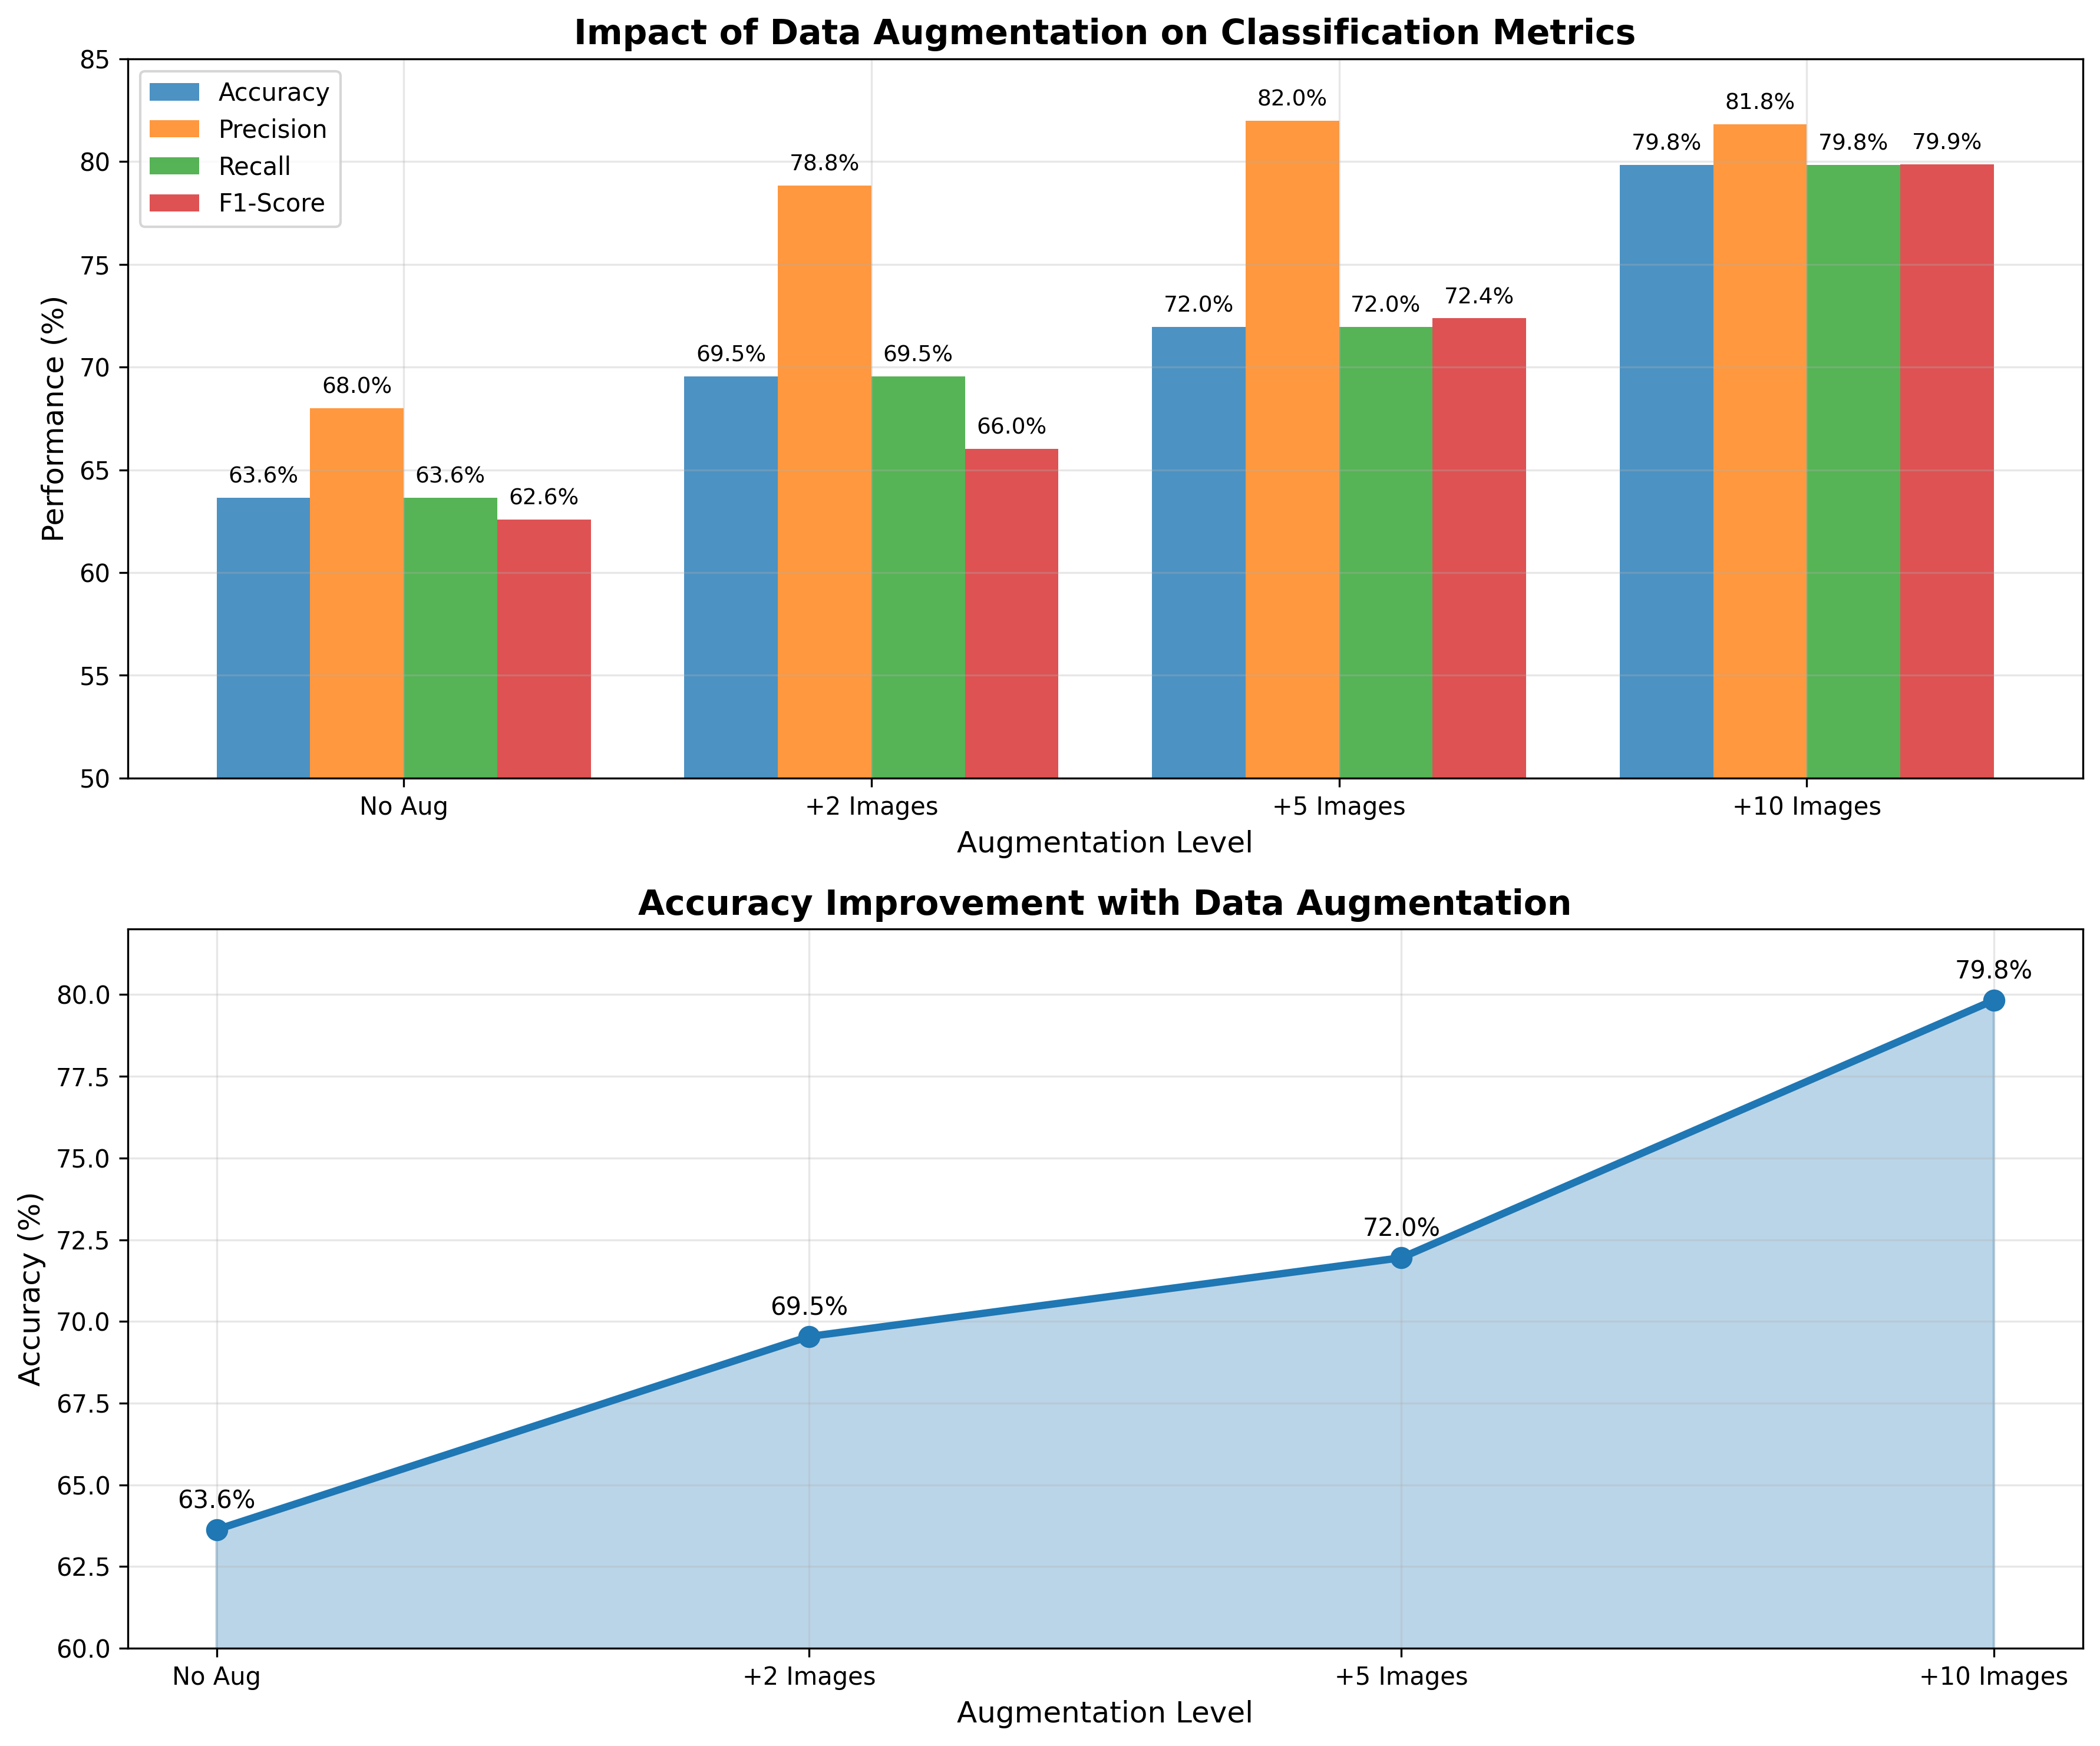
\includegraphics[width=0.9\textwidth]{../../docs/images/augmentation_impact_chart.png}
\caption{Impact of data augmentation on classification metrics. All metrics improve with additional training samples, with the steepest gain occurring between no augmentation and +2 augmentation. The accuracy trend line (orange) shows near-linear improvement initially, then plateauing around +10 augmentation.}
\label{fig:augmentation_impact}
\end{figure}

\textbf{Diminishing Returns Pattern.} The largest performance jump occurred between no augmentation and +2 augmentation (+5.91 percentage points in accuracy), while subsequent increases yielded smaller gains (+2.41 and +7.88 percentage points respectively). This suggests that even minimal augmentation significantly improves concept generalization, but returns diminish as the attractor basins stabilize.

\textbf{Few-Shot Learning Validation.} The +10 augmentation scenario achieved 79.83\% accuracy using only 5--6 unique samples per class, totaling at most 36 distinct exemplars for 6 classes. This performance is competitive with few-shot learning baselines that typically require 10--50 samples per class and multiple training epochs with backpropagation.

\subsection{Attractor Quality and Generalization}

The experimental results validate the attractor-based learning hypothesis: augmentation improves performance by expanding the parameter ranges in concept graphs, creating wider attractor basins that accept greater structural variability.

\textbf{Parametric Generalization.} With no augmentation, concepts form narrow attractors centered on the specific geometric configurations of the 5--6 seed samples. Test images with slight variations (different stroke thickness, minor rotations) fall outside these narrow parameter ranges, resulting in lower similarity scores and misclassifications. Augmentation expands these ranges: a concept trained on rotated variants learns angle ranges spanning $\pm 5^\circ$ rather than a single value, improving robustness to orientation variations in test data.

\textbf{Single-Pass Effectiveness.} All results were obtained with single-pass training (one forward traversal of the training set per class) without backpropagation or iterative weight updates. This demonstrates that energy-based structural reduction can form effective class representations without gradient descent, supporting the theoretical framework presented in the Introduction.

\section{Discussion and Limitations}

The ComAN architecture demonstrates that energy-based structural learning can achieve competitive few-shot classification without backpropagation. However, the approach exhibits distinct strengths and limitations compared to conventional neural networks.

\subsection{Strengths}

\textbf{Transparency and Interpretability.} Unlike black-box deep neural networks, ComAN concepts are explicit graph structures that can be visualized, inspected, and analyzed. Researchers can examine which structural features (endpoints, intersections, angles) contribute to classification decisions, facilitating debugging and domain knowledge validation. This interpretability is critical for applications requiring explainable AI, such as medical diagnostics or safety-critical systems.

\textbf{Few-Shot Learning Capability.} ComAN achieved 79.83\% accuracy on 6-class MNIST using only 5--6 unique exemplars per class---substantially fewer than typical deep learning approaches. Traditional CNNs often require hundreds to thousands of samples per class to achieve comparable performance, particularly when training from scratch. This data efficiency makes ComAN suitable for domains where labeled data is expensive or scarce (medical imaging, rare handwritten symbols, specialized industrial inspection).

\textbf{No Backpropagation.} The single-pass, forward-only training eliminates gradient-related pathologies (vanishing/exploding gradients, local minima, learning rate tuning). Training complexity is determined by graph operations (GED computation, clustering) rather than iterative weight optimization. This architectural simplicity may enable deployment on resource-constrained hardware where backpropagation overhead is prohibitive.

\textbf{Concept Stability.} Once formed, concept attractors remain stable---no catastrophic forgetting when exposed to new classes, as each concept is structurally independent. Adding a new class requires training a single new concept without retraining existing ones.

\subsection{Limitations}

\textbf{Scalability Concerns.} ComAN's classification complexity grows linearly with the number of classes (each test image must be matched against all concepts via GED). Graph Edit Distance computation itself is NP-hard in the general case, though practical instances with small graphs (10--30 nodes) remain tractable. Scaling to 100+ classes or complex graphs (50+ nodes) may require approximate GED algorithms or hierarchical concept organization, which remain unexplored.

\textbf{Skeletonization Dependency.} The entire pipeline depends critically on high-quality skeletonization. Errors introduced during binarization, thinning, or GNG topology learning propagate through all subsequent stages with no error correction mechanism. Unlike end-to-end learned CNNs that optimize preprocessing implicitly, ComAN's modular pipeline cannot backpropagate corrections to early stages. Low-contrast images, noisy backgrounds, or ambiguous stroke boundaries may produce malformed skeletons, degrading classification performance.

\textbf{Texture Blindness.} ComAN operates exclusively on structural topology (node/edge configurations). It cannot distinguish classes based on texture, color, or fine-grained intensity patterns. For instance, distinguishing dog breeds by fur patterns or identifying fabric types would fail entirely. This limitation restricts ComAN to structure-dominated recognition tasks.

\textbf{Limited Rotation Invariance.} While coordinate normalization provides translation invariance, ComAN exhibits limited rotation robustness. Large rotations ($>15^\circ$) alter angle parameters beyond typical parameter ranges, potentially causing misclassification. Data augmentation partially mitigates this, but fundamentally rotation-invariant feature extraction (e.g., via invariant graph kernels) remains an open challenge.

\textbf{Manual Hyperparameter Tuning.} Despite avoiding backpropagation, ComAN still requires manual tuning of multiple parameters: adaptive thresholding decrements, GNG learning rates, RDP simplification epsilon, clustering thresholds, and GED cost ratios. Automated hyperparameter optimization (grid search, Bayesian optimization) has not been explored but may improve performance.

\subsection{Comparison to Convolutional Neural Networks}

\textbf{ComAN Advantages:}
\begin{itemize}
\item Few-shot learning (5--6 samples vs 100--1000 for CNNs)
\item Interpretability (explicit graph structures vs learned weight matrices)
\item No backpropagation (simpler training, no gradient issues)
\item Concept stability (no catastrophic forgetting)
\end{itemize}

\textbf{CNN Advantages:}
\begin{itemize}
\item Superior scalability (thousands of classes, millions of samples)
\item Texture and color sensitivity (end-to-end feature learning)
\item Rotation and deformation invariance (via data augmentation and architecture)
\item State-of-the-art accuracy on standard benchmarks (95--99\% on full MNIST)
\end{itemize}

\textbf{Complementary Paradigms.} ComAN and CNNs address different problem classes. CNNs excel at large-scale, data-rich, texture-sensitive tasks where interpretability is secondary. ComAN targets small-data, structure-dominated, interpretability-critical applications. Hybrid approaches---using CNNs for feature extraction followed by ComAN-style structural matching---may combine strengths of both paradigms.

\section{Conclusions and Future Work}

\subsection{Summary}

We presented the Compartment Attractor Neural Network (ComAN), a novel architecture for few-shot structural classification that replaces backpropagation-based learning with energy-based attractor formation. The system transforms images into graph representations through skeletonization and topology learning, then iteratively forms concept attractors through Lyapunov-driven structural and parametric reduction operators. Classification proceeds by reducing test graphs toward stored attractors and selecting the nearest match via Winner-Takes-All competition based on Graph Edit Distance.

Experimental validation on a 6-class MNIST subset demonstrated competitive few-shot performance: 79.83\% accuracy using only 5--6 unique training exemplars per class (36 total unique samples), trained in a single forward pass without backpropagation. This represents a viable alternative to gradient-descent-based learning for structure-dominated pattern recognition tasks where interpretability and data efficiency are priorities.

\subsection{Contributions}

The primary contributions of this work include:

\begin{enumerate}
\item \textbf{Energy-based structural learning framework:} A theoretically grounded approach to concept formation based on internal energy minimization rather than external error minimization, eliminating backpropagation and its associated pathologies.

\item \textbf{Graph-based concept representation:} An explicit, inspectable representation of class knowledge as attributed graphs with parametric ranges, enabling visualization and interpretation of learned concepts.

\item \textbf{Lyapunov-driven reduction operators:} A suite of structural and parametric reduction operators that implement gradient descent along energy landscapes through graph transformations, validated empirically on handwritten digit recognition.

\item \textbf{Few-shot learning validation:} Empirical demonstration that energy-based attractor formation can achieve competitive classification performance (80\% accuracy) using minimal training data (5--6 samples per class), supporting the hypothesis that structural self-organization offers advantages over statistical learning for small-data regimes.
\end{enumerate}

\subsection{Future Directions}

Several promising research directions emerge from this work:

\textbf{Scalability Evaluation.} Test ComAN on larger-scale datasets with more classes: EMNIST (47 balanced classes, 112,800 training images) to evaluate multi-class scaling; Quick, Draw! (345 classes, millions of sketches) to test extreme-scale concept organization. Investigate hierarchical concept structures or approximate GED algorithms to manage computational complexity.

\textbf{Computational Optimization.} Explore approximate GED algorithms (e.g., graph kernel methods, learned graph embeddings) to reduce classification time from $O(|V|^3)$ per concept to sublinear complexity. Investigate GPU acceleration of graph operations and parallel concept matching to enable real-time classification.

\textbf{Automated Hyperparameter Tuning.} Develop principled methods for selecting clustering parameters, GED cost ratios, and simplification thresholds. Apply Bayesian optimization or evolutionary algorithms to learn optimal parameter configurations for specific datasets, reducing manual tuning requirements.

\textbf{Hierarchical Concept Maps.} Extend the single-attractor-per-class model to hierarchical ``neuron maps'' that capture intra-class variability. For example, represent digit ``7'' as a collection of sub-attractors: one for crossed sevens, one for uncrossed sevens, enabling finer-grained recognition and probabilistic confidence estimation.

\textbf{Rotation Invariance.} Investigate rotation-invariant graph features (e.g., spectral graph descriptors, persistent homology) or equivariant graph neural networks to achieve robustness to arbitrary rotations without exhaustive data augmentation.

\textbf{Hybrid Architectures.} Explore combinations of deep learning and structural matching: use CNNs for robust feature extraction and skeletonization, then apply ComAN-style graph matching for interpretable classification. Such hybrid systems may leverage the complementary strengths of both paradigms.

\section{References}

\bibliographystyle{IEEEtran}
\begin{thebibliography}{99}

\bibitem{rumelhart1986}
D.~E. Rumelhart, G.~E. Hinton, and R.~J. Williams, ``Learning representations by back-propagating errors,'' \emph{Nature}, vol.~323, pp. 533--536, Oct. 1986.

\bibitem{hochreiter2001}
S.~Hochreiter, Y.~Bengio, P.~Frasconi, and J.~Schmidhuber, ``Gradient flow in recurrent nets: The difficulty of learning long-term dependencies,'' in S.~C. Kremer and J.~F. Kolen (eds.), \emph{A Field Guide to Dynamical Recurrent Neural Networks}. Piscataway, NJ, USA: IEEE Press, 2001, pp. 237--243.

\bibitem{lipton2018}
Z.~C. Lipton, ``The mythos of model interpretability,'' \emph{Queue}, vol.~16, no.~3, pp. 31--57, Jun. 2018.

\bibitem{dietterich1995}
T.~G. Dietterich, ``Overfitting and undercomputing in machine learning,'' \emph{ACM Computing Surveys}, vol.~27, no.~3, pp. 326--327, Sep. 1995.

\bibitem{kaplan2020}
J.~Kaplan, S.~McCandlish, T.~Henighan, T.~B. Brown, B.~Chess, R.~Child, S.~Gray, A.~Radford, J.~Wu, and D.~Amodei, ``Scaling laws for neural language models,'' \emph{arXiv preprint} arXiv:2001.08361, 2020.

\bibitem{crick1989}
F.~Crick, ``The recent excitement about neural networks,'' \emph{Nature}, vol.~337, pp. 129--132, Jan. 1989.

\bibitem{strubell2019}
E.~Strubell, A.~Ganesh, and A.~McCallum, ``Energy and policy considerations for deep learning in NLP,'' in \emph{Proceedings of the 57th Annual Meeting of the Association for Computational Linguistics}, 2019, pp. 3645--3650.

\bibitem{thompson2020}
S.~Thompson, K.~Greenewald, K.~Lee, and G.~F. Manso, ``The computational limits of deep learning,'' \emph{arXiv preprint} arXiv:2007.05558, 2020.

\bibitem{patterson2021}
D.~Patterson, J.~Gonzalez, Q.~Le, C.~Liang, L.~M. Munguia, D.~Rothchild, D.~So, M.~Texier, and J.~Dean, ``Carbon emissions and large neural network training,'' \emph{arXiv preprint} arXiv:2104.10350, 2021.

\bibitem{ji2023}
Z.~Ji, N.~Lee, R.~Frieske, T.~Yu, D.~Su, Y.~Xu, E.~Ishii, Y.~J. Bang, A.~Madotto, and P.~Fung, ``Survey of hallucination in natural language generation,'' \emph{ACM Computing Surveys}, vol.~55, no.~12, pp. 1--38, 2023.

\bibitem{huang2023}
L.~Huang, W.~Yu, W.~Ma, W.~Zhong, Z.~Feng, H.~Wang, Q.~Chen, W.~Peng, X.~Feng, B.~Qin, and T.~Liu, ``A survey on hallucination in large language models: Principles, taxonomy, challenges, and open questions,'' \emph{arXiv preprint} arXiv:2311.05232, 2023.

\bibitem{shumailov2023}
I.~Shumailov, Z.~Shumaylov, Y.~Zhao, Y.~Gal, N.~Papernot, and R.~Anderson, ``The curse of recursion: Training on generated data makes models forget,'' \emph{arXiv preprint} arXiv:2305.17493, 2023.

\bibitem{alemohammad2023}
S.~Alemohammad, J.~Casco-Rodriguez, L.~Luzi, A.~I. Humayun, H.~Babaei, D.~LeJeune, A.~Siahkoohi, and R.~G. Baraniuk, ``Self-consuming generative models go MAD,'' \emph{arXiv preprint} arXiv:2307.01850, 2023.

\bibitem{landauer1961}
R.~Landauer, ``Irreversibility and heat generation in the computing process,'' \emph{IBM Journal of Research and Development}, vol.~5, no.~3, pp. 183--191, 1961.

\bibitem{hopfield1982}
J.~J. Hopfield, ``Neural networks and physical systems with emergent collective computational abilities,'' \emph{Proceedings of the National Academy of Sciences}, vol.~79, no.~8, pp. 2554--2558, 1982.

\bibitem{hubel1968}
D.~H. Hubel and T.~N. Wiesel, ``Receptive fields and functional architecture of monkey striate cortex,'' \emph{The Journal of Physiology}, vol.~195, no.~1, pp. 215--243, 1968.

\bibitem{deraedt2008}
L.~De Raedt, \emph{Logical and Relational Learning}. Berlin, Germany: Springer, 2008.

\bibitem{latecki1998}
L.~J. Latecki and R.~Lakaemper, ``Shape similarity measure based on correspondence of visual parts,'' \emph{IEEE Trans. Pattern Anal. Mach. Intell.}, vol.~22, no.~10, pp. 1185--1190, 2000.

\bibitem{lam1997}
L.~Lam and C.~Y.~Suen, ``An evaluation of parallel thinning algorithms for character recognition,'' \emph{IEEE Trans. Pattern Anal. Mach. Intell.}, vol.~17, no.~9, pp. 914--919, 1995.

\bibitem{fritzke1995}
B.~Fritzke, ``A growing neural gas network learns topologies,'' in \emph{Advances in Neural Information Processing Systems}, vol.~7, Morgan Kaufmann, 1995, pp. 625--632.

\bibitem{huang2006}
G.-B. Huang, Q.-Y. Zhu, and C.-K. Siew, ``Extreme learning machine: Theory and applications,'' \emph{Neurocomputing}, vol.~70, no.~1--3, pp. 489--501, Dec. 2006.

\bibitem{jaeger2001}
H.~Jaeger, ``The `echo state' approach to analysing and training recurrent neural networks,'' GMD Report 148, German National Research Center for Information Technology, 2001.

\bibitem{parzhin2025}
Y.~Parzhin, M.~Lapin, and K.~Bokhan, ``A new approach to building energy models of neural networks,'' \emph{Energy-Based Neural Network Modeling}, preprint, 2025.

\end{thebibliography}


\appendix

\section{Reduction Rule Schemata}

This appendix provides visual illustrations of the key structural reduction rules applied during concept formation and classification.

\subsection{IntersectionPoint to CornerPoint Reduction}

\begin{figure}[h]
\centering
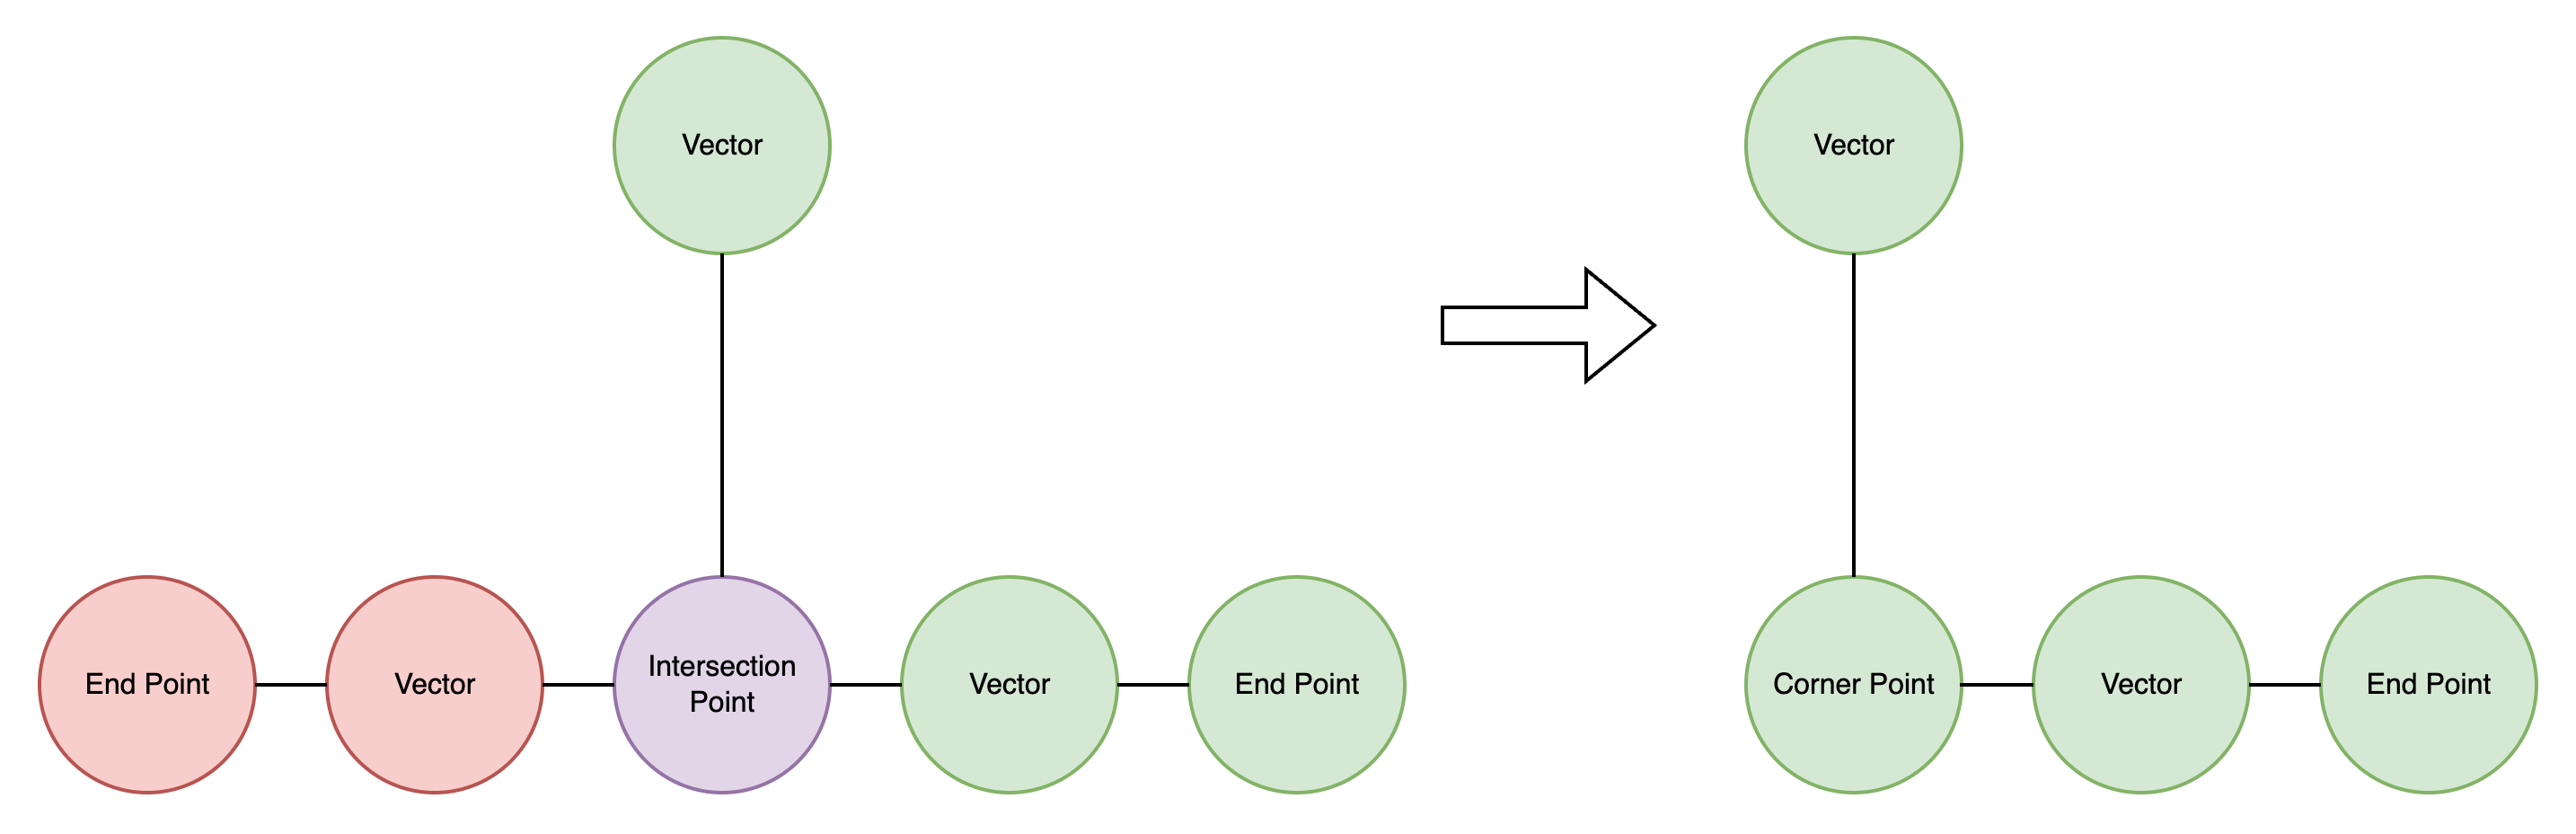
\includegraphics[width=0.7\textwidth]{../../docs/images/intersection_point_to_corner_point.png}
\caption{Reduction of IntersectionPoint to CornerPoint. When structural reduction removes edges from an intersection point such that the degree no longer matches the expected intersection degree (typically $\deg(v) \geq 3$), the point is demoted to CornerPoint. This preserves topological information while simplifying node type classifications.}
\label{fig:intersection_corner}
\end{figure}

\subsection{IntersectionPoint to EndPoint Reduction}

\begin{figure}[h]
\centering
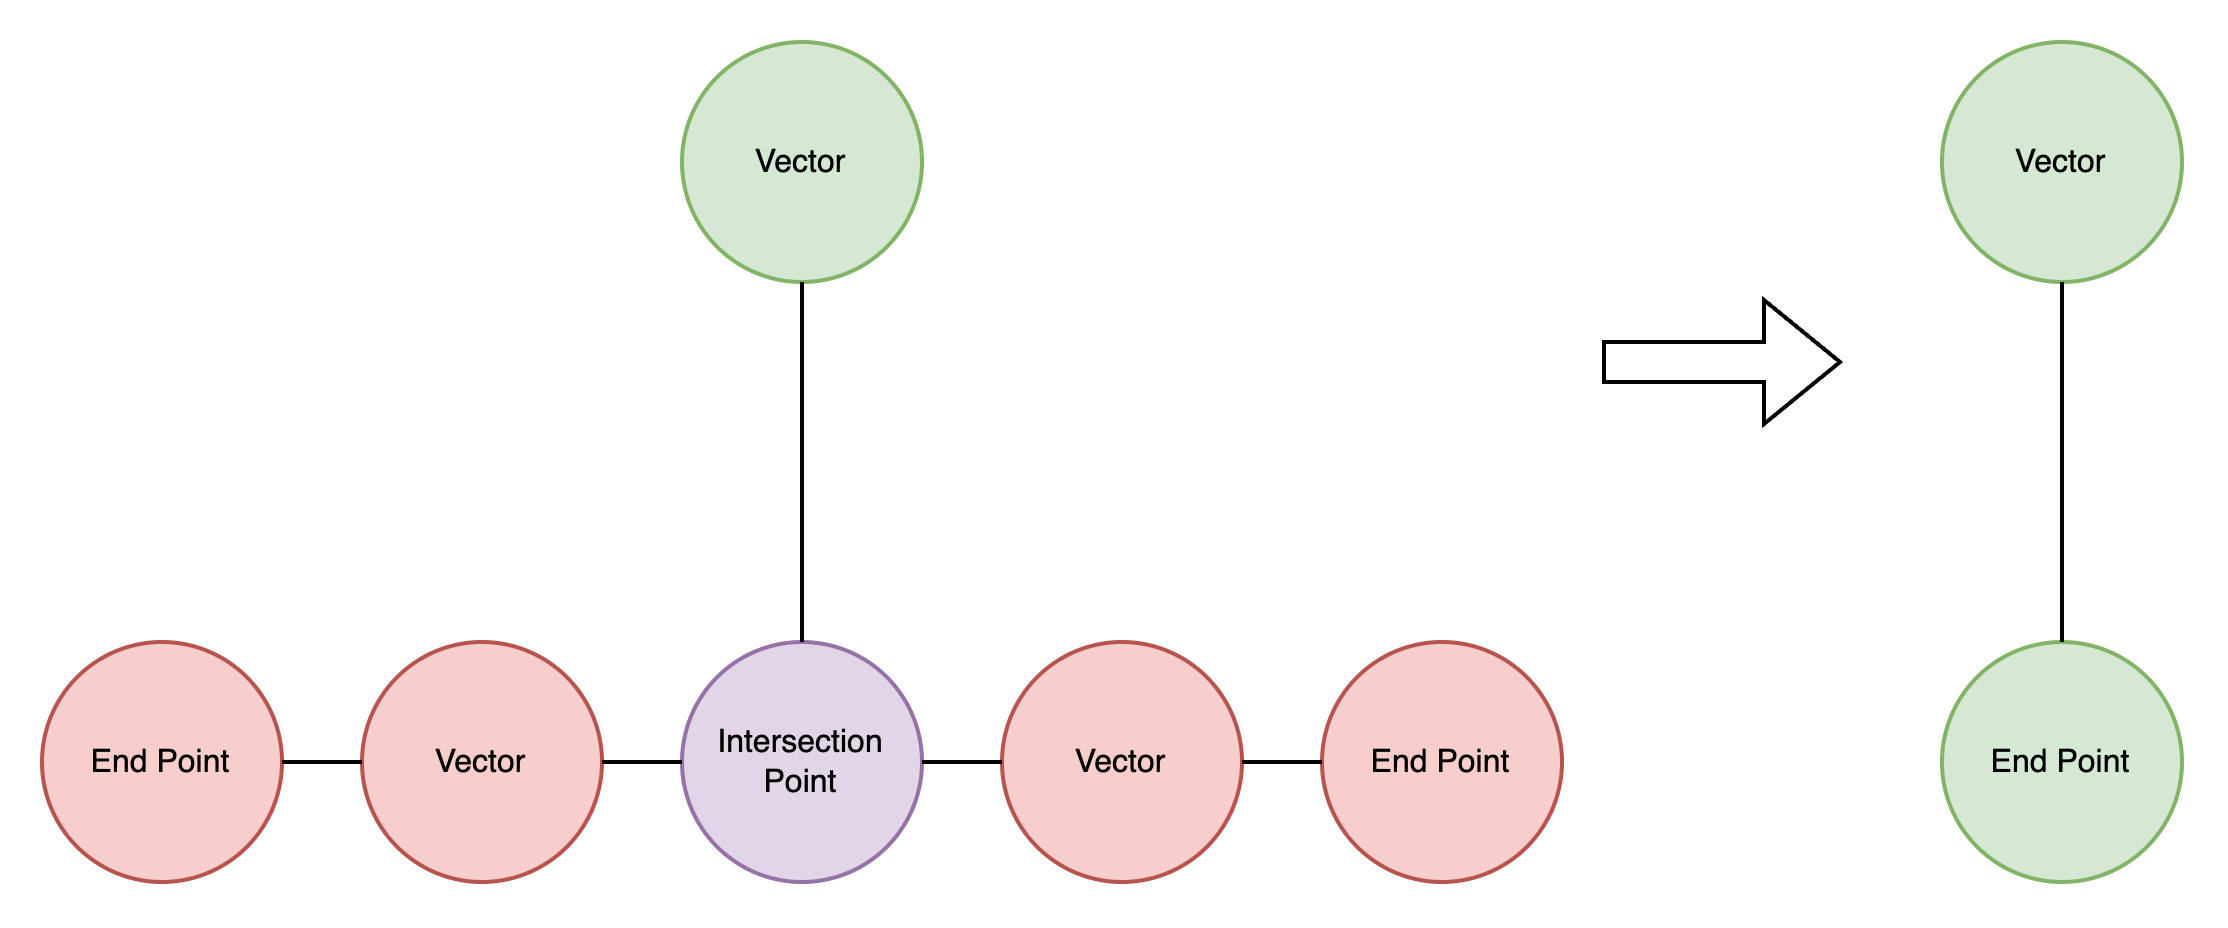
\includegraphics[width=0.7\textwidth]{../../docs/images/intersection_point_to_endpoint.png}
\caption{Reduction of IntersectionPoint to EndPoint. If edge removal reduces an intersection point's degree to 1, the point is reclassified as an EndPoint. This occurs when branches are pruned during structural alignment, leaving a former intersection as a terminal node.}
\label{fig:intersection_endpoint}
\end{figure}

\section{Example Concept Formation}

Figure~\ref{fig:concept_example} demonstrates the iterative concept formation process for MNIST digit ``3'', showing the structural evolution from initial seed to final generalized attractor.

\begin{figure}[h]
\centering
\begin{minipage}{0.45\textwidth}
\centering
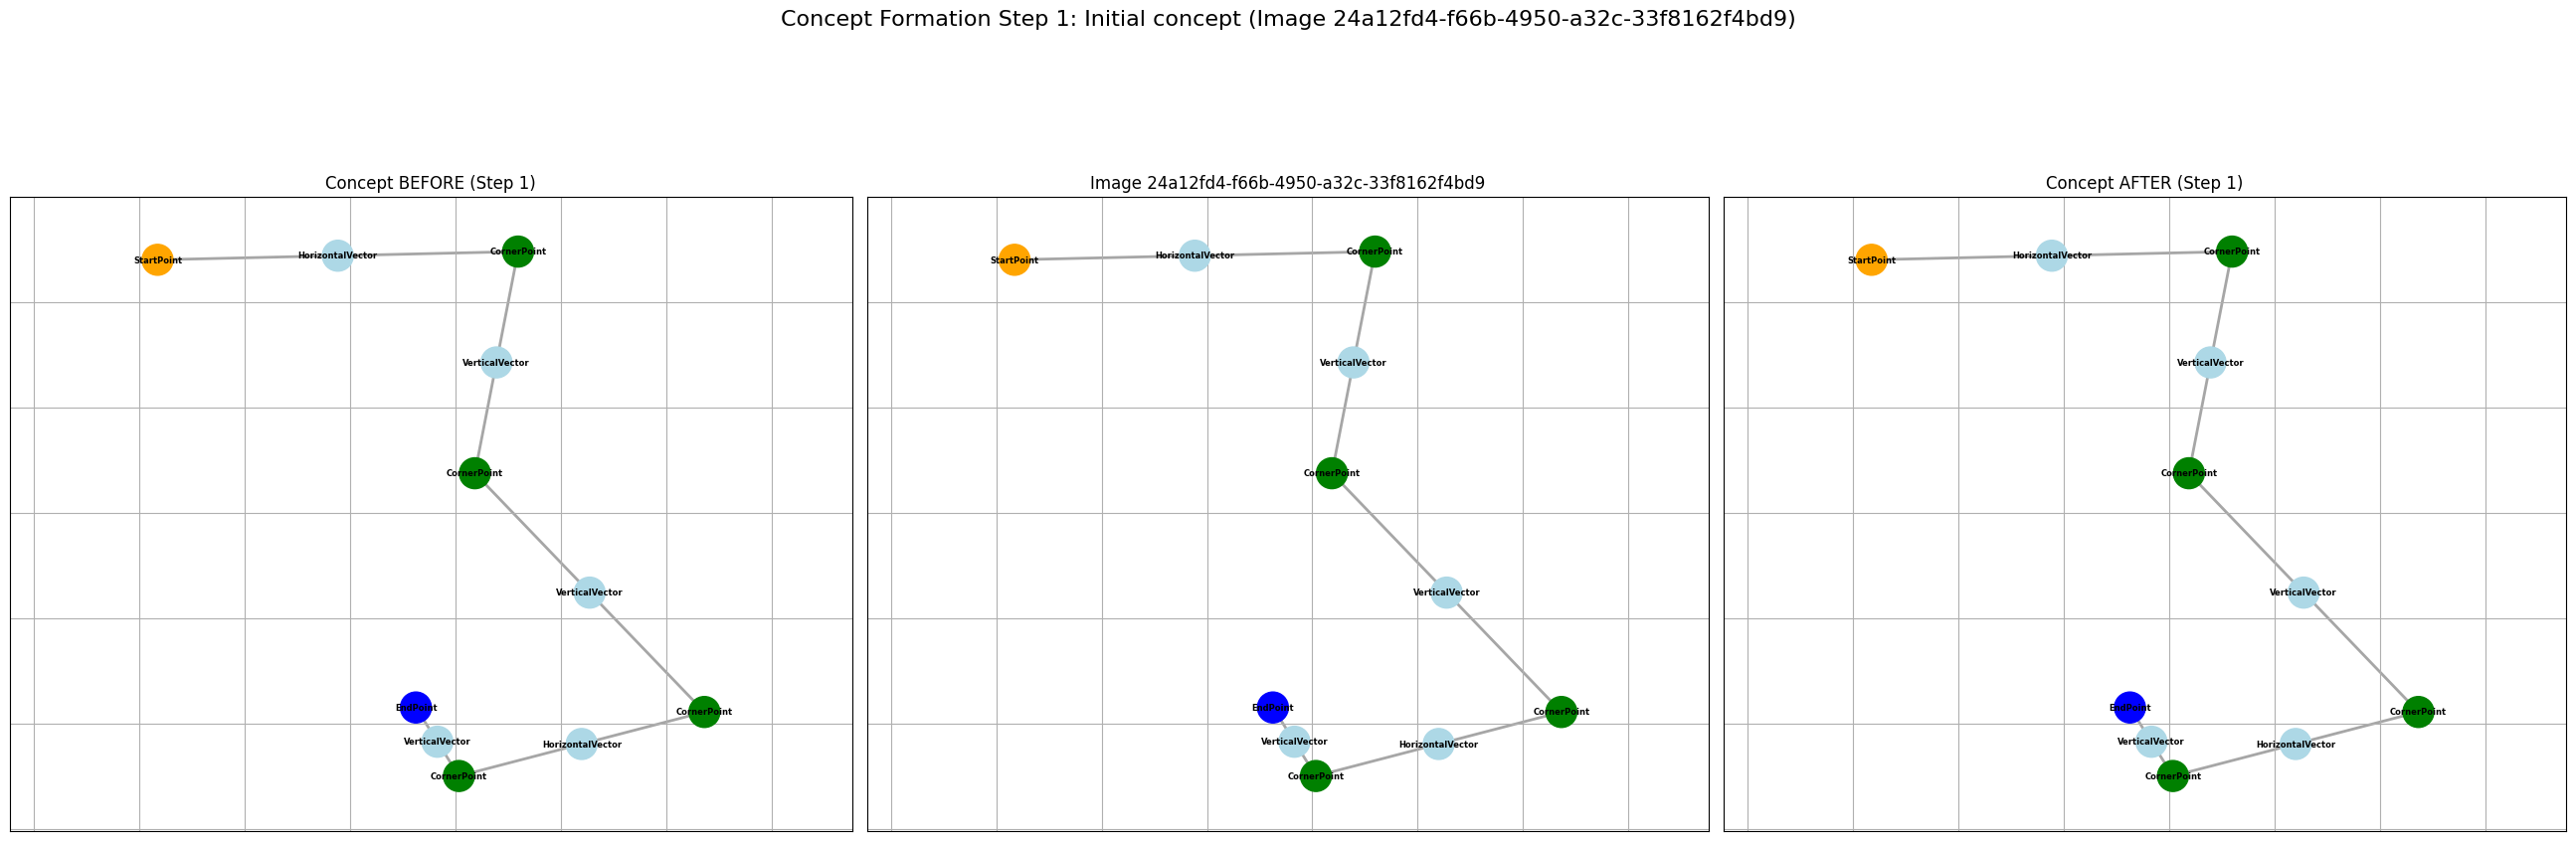
\includegraphics[width=\textwidth]{../../docs/images/concept_formation/step_1.png}
\subcaption{Initial seed: $C_0 = G_1$}
\end{minipage}
\hfill
\begin{minipage}{0.45\textwidth}
\centering
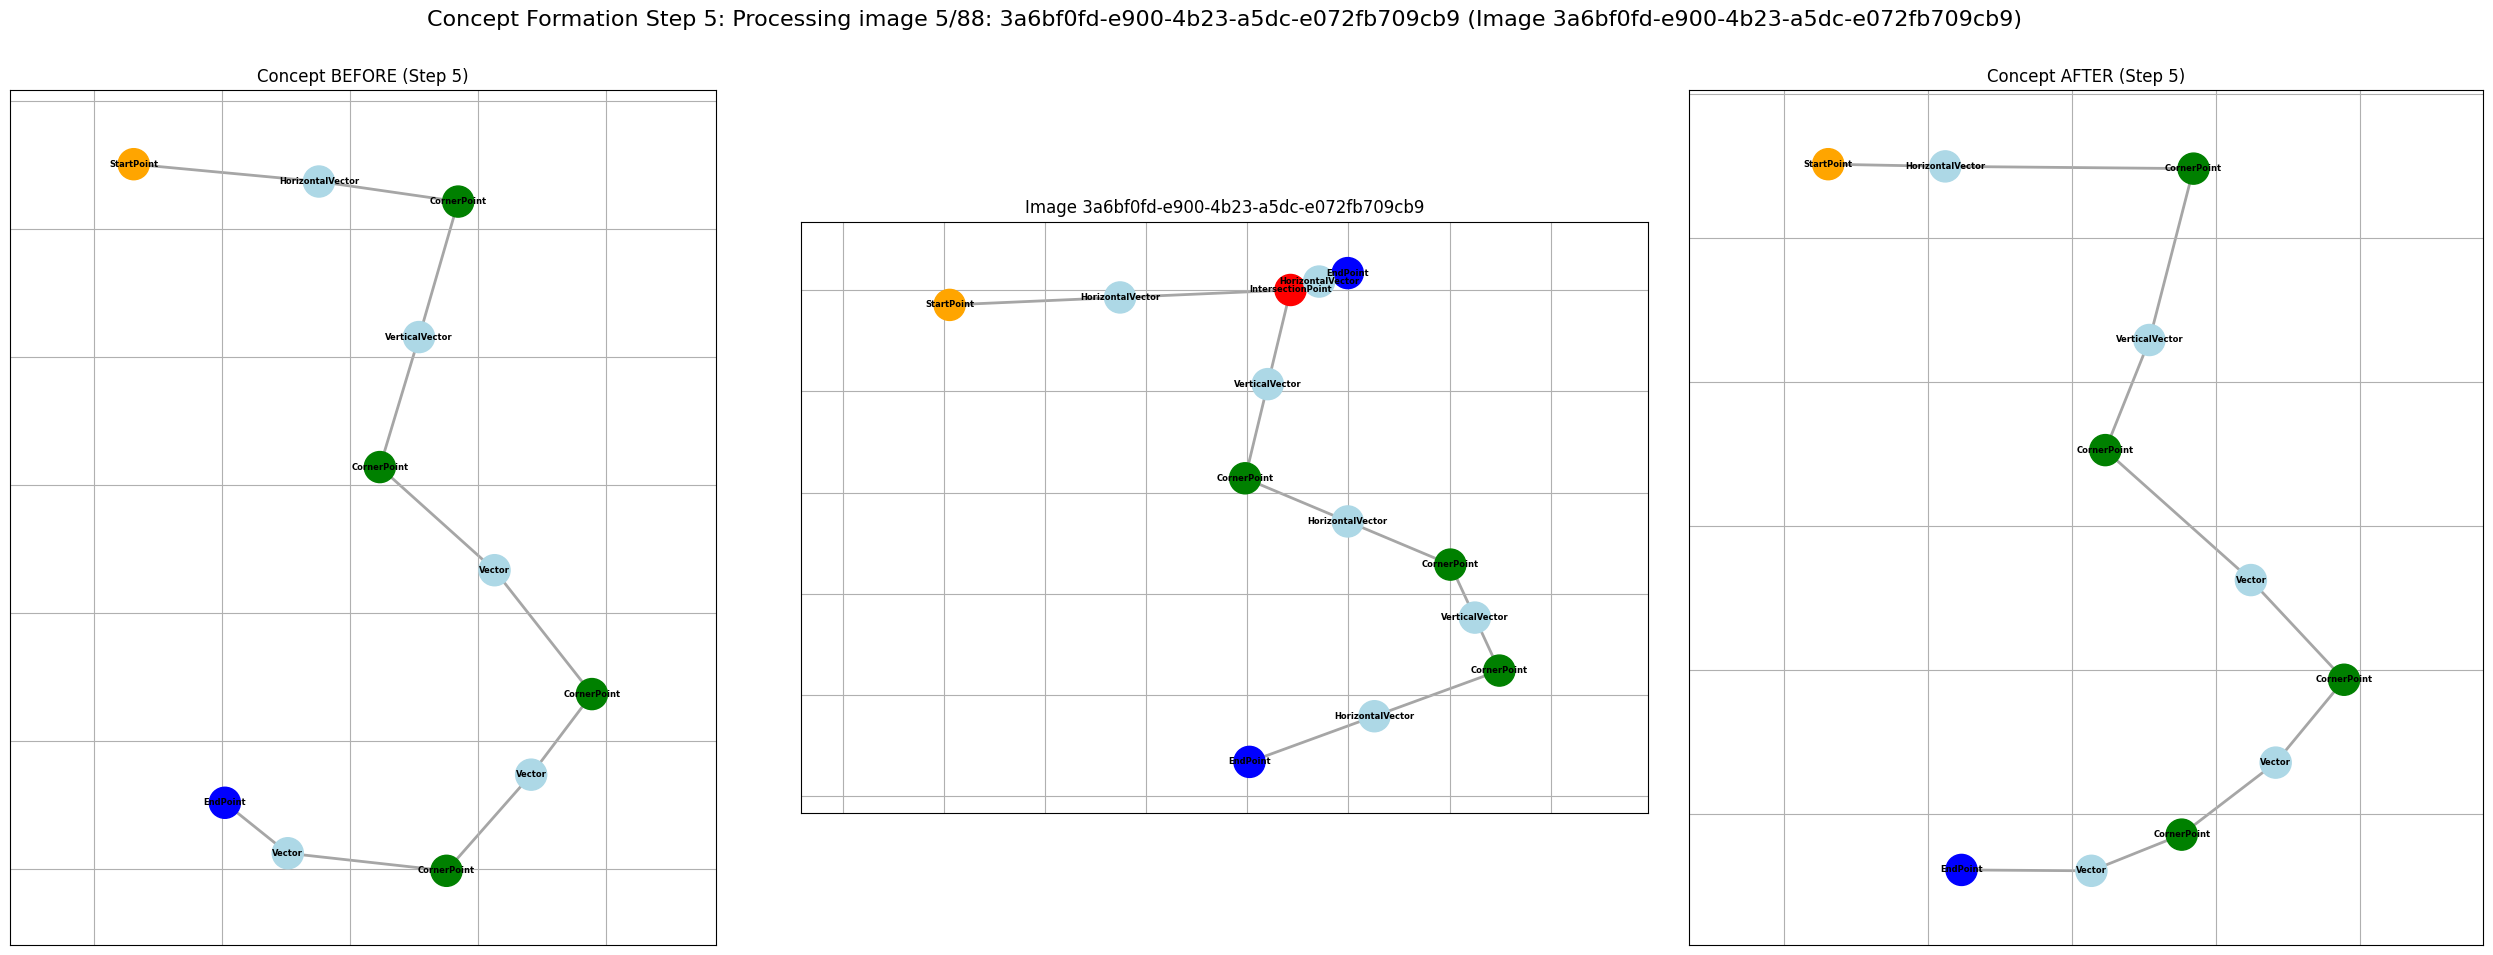
\includegraphics[width=\textwidth]{../../docs/images/concept_formation/step_4.png}
\subcaption{Final concept after 4 iterations}
\end{minipage}
\caption{Concept formation progression for digit ``3''. (a) The first training sample serves as the initial concept with precise geometric parameters. (b) After processing 4 training samples, the concept graph simplifies structurally (fewer nodes) while generalizing parametrically (angle ranges, expanded position bounds). Blue indicates concept structure; red shows training samples during reduction.}
\label{fig:concept_example}
\end{figure}

The transformation illustrates three key mechanisms: (1) endpoint pruning removes structural noise, (2) intersection-to-corner reduction simplifies node types, and (3) parametric generalization expands acceptable value ranges, creating a wider attractor basin that accepts greater intra-class variability while preserving essential topological structure.

\end{document}
